% Dokumentinformationen
%Vorlage erstellt von Luca Mazzoleni aufbaudend auf der Vorlage von Stefan Reinli

% !TeX program = pdflatex
% !TeX encoding = utf8
% !TeX spellcheck = de_DE
% !BIB program = bibtex

\documentclass[
11pt,
final,
oneside,
a4paper]{article}
%%%%

% Document information
\newcommand*{\Title}            {Geschwindigkeitserfassung Ballwurfmaschiene}
\newcommand*{\TitleInfo}        {Projektarbeit HS18}
\newcommand*{\AuthorOne}		{Luca Mazzoleni}
\newcommand*{\AuthorTwo}		{}
\newcommand*{\Author}			{\AuthorOne}
\newcommand*{\Prof}				{Markus Kottmann}
\newcommand*{\Modul}			{Einf\"uhrung Programmierung}
\newcommand*{\Betreuer}			{Daniel Raillard}
\newcommand*{\Place}            {Rapperswil}
\newcommand*{\LogoHSR}          {
\includegraphics[height = 1cm]{header/hsrlogo}}
\newcommand*{\LogoCompany}      {}
\newcommand*{\Print}            {false} % true for black links (print version), false for color links (pdf version)

% Header
\usepackage[T1]{fontenc}	% ä,ü...
\usepackage[utf8]{inputenc} % utf-8 Unterstützung
\usepackage[ngerman]{babel} % Silbentrennung und Rechtschreibung Deutsch
\usepackage[{left=1.5cm,right=1.5cm,top=0cm,bottom=0cm}]{geometry} % Seitenränder Titelblatt


%%%%%%%%%%%%%%%%%%%%%%%
%% Packages
%%%%%%%%%%%%%%%%%%%%%%%
\usepackage[page,header]{appendix}
\usepackage{acronym} 		   % Für Abkürzungsverzeichnis
\usepackage{adjustbox} 		   % adjustbox, minipage..
\usepackage{amsmath}   		   % Allgemeine Matheumgebungen
\usepackage{amssymb}  		   % Fonts: msam,msbm, eufm & Mathesymbole, Mengen (lädt automatisch amsfonts)
\usepackage{array} 			   % Extending the array and tabular environment -> m,b,p,..
\usepackage{caption}  		   % Verändern der Schriftart von Bildunterschriften
\usepackage{changepage}
\usepackage{epstopdf}
\usepackage{expl3}
\usepackage{float}
\usepackage{framed, color}
\usepackage{fancyhdr}			%Für Kopf & Fusszeile
\usepackage{graphbox}
\usepackage{graphicx}
\usepackage{titletoc}			% Editieren des TOCs muss vor hyperref geladen werden
\usepackage{tocloft}			% Editieren des TOCs muss vor hyperref geladen werden
\usepackage{hyperref}
\usepackage{hyphenat}			%Wortumbruch
\hyphenation{he-lio-trope opos-sum}

\usepackage{listings}           % Erlaubt es Programmcode in der gewünschten Sprache zu hinterlegen (C++, Matlab,..)
\usepackage{longtable}
\usepackage{lastpage}			%Lastpage ref for Footer
\usepackage{marginnote} 		% Für Seitenkommentare \marginnote
\usepackage{mathtools}          % Vor mathabx laden!
\usepackage{mathabx} 			% Package mit vielen weiteren Mathe Symbolen
\usepackage{mparhack}  			% Improved marginpar placement
\usepackage{multicol} 			% In­ter­mix sin­gle and mul­ti­ple columns
\usepackage{multirow} 			% Create tabular cells spanning multiple rows
\usepackage{paralist}
\usepackage{pdfpages} 
\usepackage{pxfonts} 			% Mathsymbols
\usepackage[section]{placeins}  % Float-Barrier for Section
\usepackage{rotating} 			% Rotation tools, including rotated fullpage floats
\usepackage[onehalfspacing]{setspace}
\usepackage{scrhack}        	% Fixes koma-script incompatibilities
\usepackage{subcaption}
\usepackage{tabularx}
\usepackage{textcomp} 			% Wird für Copyright-Symbol,Währungen, Musikalische-Symbole benötigt
\usepackage[colorinlistoftodos,prependcaption,textsize=tiny]{todonotes}
\usepackage[most]{tcolorbox}
\usepackage{trfsigns}
\usepackage{varwidth}
\usepackage{wrapfig}

%%%%%%%%%%%%%%%%%%%%%%%
%% PDF Meta Data
%%%%%%%%%%%%%%%%%%%%%%%

\hypersetup{pdftex,
pdfauthor={\Author},
pdftitle={\Title},
pdfsubject={\TitleInfo},
%pdfkeywords={Some Keywords},
pdfproducer={Latex with hyperref}
%pdfcreator={pdflatex}
}

%%%%%%%%%%%%%%%%%%%%%%%
%% Setup Tikz
%%%%%%%%%%%%%%%%%%%%%%%
%\usepackage{tikz}
%\usepackage{struktex}
%\usepackage{schemabloc}
%\usepackage[normalem]{ulem}
%\usetikzlibrary{circuits}
%\usetikzlibrary{arrows}
%\usetikzlibrary{circuits.ee.IEC}
%\usetikzlibrary{patterns}
%\usetikzlibrary{positioning}
%\usetikzlibrary{shapes,arrows}
%
%\usepackage{pgfplots}
%\usepackage{pgfplotstable}
%\pgfplotsset{compat=newest}
%
%\tikzstyle{block} = [draw, rectangle, minimum height=3em, minimum width=4em]
%\tikzstyle{input} = [coordinate]
%\tikzstyle{output} = [coordinate]
%\tikzstyle{pinstyle} = [pin edge={to-,thin,black}]
%\tikzstyle{sum} = [draw, circle, node distance=1em, minimum height=1.5em]
%\tikzset{>=latex}
%\tikzset{%
%	block/.style    = {draw, thick, rectangle, minimum height = 3em,
%		minimum width = 3em},
%	sum/.style      = {draw, circle, node distance = 1.5cm}, % Adder
%	input/.style    = {coordinate}, % Input
%	output/.style   = {coordinate} % Output
%}
%\newcommand\Umbruch[2][3cm]{\begin{varwidth}{#1}\centering#2\end{varwidth}}

%%%%%%%%%%%%%%%%%%%%%%%
% Caption Setup
%%%%%%%%%%%%%%%%%%%%%%%
\captionsetup[figure]{labelfont={it,bf},textfont={it}}
\captionsetup[table]{labelfont={it,bf},textfont={it},singlelinecheck=off,justification=centering}
\captionsetup[lstlisting]{labelfont={it,bf},textfont={it}}
\captionsetup[subfigure]{labelfont=bf,textfont=normalfont,singlelinecheck=off,justification=centering}

\newenvironment{nscenter}
{\parskip=-5pt\par\nopagebreak\centering}
{\parskip=-15pt\par\noindent\ignorespacesafterend}

%Rewritte Referenze Style and TOF,TOT
\renewcommand{\thefigure}{Abb. \arabic{figure}}
\renewcommand{\thetable}{Tab. \arabic{table}}
\renewcommand{\theequation}{Formel \arabic{equation}}

\addto{\captionsngerman}{%
    %	\renewcommand*{\contentsname}{Inhalt}
    %	\renewcommand*{\listfigurename}{Abbildungen}
    %	\renewcommand*{\listtablename}{Tabellen}
    \renewcommand*{\figurename}{} %Delet Figure name 
    \renewcommand*{\tablename}{}
}
\setlength{\cftfignumwidth}{2cm}	% Width of equation number in List of Figure
\setlength{\cfttabnumwidth}{2cm}	% Width of equation number in List of Table

%List of Equations
\newcommand{\listequationsname}{Gleichungen}
\newlistof{myequations}{equ}{\listequationsname}
\newcommand{\myequations}[1]{% 
    \addcontentsline{equ}{myequations}{\protect\numberline{\theequation}#1}\par}
\setlength{\cftmyequationsnumwidth}{2cm}% Width of equation number in List of Equations


%%%%%%%%%%%%%%%%%%%%%%%%
%% Header and Footer %%
%%%%%%%%%%%%%%%%%%%%%%%%
\pagestyle{fancy} %eigener Seitenstil
\renewcommand{\sectionmark}[1]{\markright{#1}} %entfernt nummer vor section
\renewcommand{\subsectionmark}[1]{}
%twopage
%\ifthenelse{\isodd{\value{page}}}{\leftmark}{\rightmark}
% or with
%\fancyhead[OR]{} % "O" for "odd"
%\fancyhead[ER]{} % "E" for "even"

\fancypagestyle{plain}{
    \fancyhf{} %alle Kopf- und Fußzeilenfelder bereinigen
    
    \fancyhead[OR]{\LogoHSR}
    \fancyhead[ER]{\LogoCompany}
    \fancyhead[C]{\textsl{\rightmark}} %zentrierte Kopfzeile
    \fancyhead[OL]{\LogoCompany}
    \fancyhead[EL]{\LogoHSR}
    \renewcommand{\headrulewidth}{0.4pt} %obere Trennlinie
    
    \fancyfoot[OR]{Seite \thepage\ / \pageref{LastPage}}
    \fancyfoot[ER]{\today}
    \fancyfoot[C]{\small{\Author}}
    \fancyfoot[EL]{Seite \thepage\ / \pageref{LastPage}}
    \fancyfoot[OL]{\today}
    \renewcommand{\footrulewidth}{0.4pt} %untere Trennlinie
}

\fancypagestyle{appendix}{
    \fancyhf{} %alle Kopf- und Fußzeilenfelder bereinigen
    \fancyhead[R]{} %Kopfzeile links
    \fancyhead[C]{} %zentrierte Kopfzeile
    \fancyhead[L]{} %Kopfzeile rechts
    \renewcommand{\headrulewidth}{0pt} %obere Trennlinie
    
    \fancyfoot[OR]{Seite \thepage\ / \pageref{LastPage}}
    \fancyfoot[ER]{\today}
    \fancyfoot[C]{}
    \fancyfoot[EL]{Seite \thepage\ / \pageref{LastPage}}
    \fancyfoot[OL]{\today}
    \renewcommand{\footrulewidth}{0.4pt} %untere Trennlinie
}


\pagestyle{plain} %Pagesytle


%%%%%%%%%%%%%%%%%%%%%
%% Load HSR Color  %%
%%%%%%%%%%%%%%%%%%%%%
\usepackage{xcolor}
\usepackage{header/HSRColors}

%%%%%%%%%%
% Colors %
%%%%%%%%%%
\definecolor{black}{rgb}{0,0,0}
\definecolor{red}{rgb}{1,0,0}
\definecolor{white}{rgb}{1,1,1}
\definecolor{grey}{rgb}{0.8,0.8,0.8}
\definecolor{green}{rgb}{0,.8,0.05}
\definecolor{brown}{rgb}{0.603,0,0}
\definecolor{mymauve}{rgb}{0.58,0,0.82}
\definecolor{mygreen}{RGB}{28,172,0}
\definecolor{mygray}{rgb}{0.5,0.5,0.5}
\definecolor{mymauve}{rgb}{0.58,0,0.82}
\definecolor{mylilas}{RGB}{170,55,241}

\definecolor{gray80}{gray}{0.8}
\definecolor{gray60}{gray}{0.6}
\definecolor{gray40}{gray}{0.4}
\definecolor{gray20}{gray}{0.2}

%%%%%%%%%%%%%%%%%%%%%
%% Title %%
%%%%%%%%%%%%%%%%%%%%%



%Title Spacing-----------------------------------------
\usepackage{titlesec}
%\titlespacing{name=\section}{-\marginparwidth}{0pt}{0.2em}
%\titlespacing{name=\subsection}{-\marginparwidth+10pt}{0pt}{0.2em}
%\titlespacing{name=\subsubsection}{-\marginparwidth+14pt}{0.2em}{0.2em}
%\titlespacing{name=\paragraph}{-\marginparwidth+18pt}{0.2em}{0.2em}

\titlespacing{name=\section}{1pt}{0pt}{0.2em}
\titlespacing{name=\subsection}{1pt}{0pt}{0.2em}
\titlespacing{name=\subsubsection}{1pt}{0.2em}{0.2em}
\titlespacing{name=\paragraph}{1pt}{0.2em}{0.2em}

%%%%%%%%%%%%%%%%%%
%% Bibliography %%
%%%%%%%%%%%%%%%%%%
%\usepackage[fixlanguage]{babelbib}
%\selectbiblanguage{german}
\usepackage[backend=bibtex,style=ieee, defernumbers=true]{biblatex} %Do not use biber with TexWorks
\addbibresource{Literatur}


% Abbildungen im Quellenverzeichnis nach Alphabet ordnen, Rest nummerieren
%\DeclareFieldFormat{labelnumber}{\ifkeyword{abb}{\mknumalph{#1}}{#1}}


%%%%%%%%%%%%%%%%%%%%%%%%%%%%%%%%%%%
%% Itemize and Enumerate spacing %%
%%%%%%%%%%%%%%%%%%%%%%%%%%%%%%%%%%%
% \topsep: space between first item and preceding paragraph
% \partopsep: extra space added to \topsep when environment starts a new paragraph
% \itemsep: space between successive items. 
\usepackage{enumitem} % Controls Layout of itemize, enumerate, description
\setlist[itemize]{topsep=0pt,itemsep=-1ex,partopsep=1ex,parsep=1ex,after=\vskip0.1\baselineskip}
\setlist[enumerate]{topsep=0pt,itemsep=-1ex,partopsep=1ex,parsep=1ex,after=\vskip0.1\baselineskip}

%%%%%%%%%%%
%% Index %%
%%%%%%%%%%%
\usepackage{imakeidx}
\makeindex[intoc,columnseprule]
\indexsetup{firstpagestyle=plain}    % Show header/footer on index page

%-------------------------------------------------
% Marginalien/Seitenränder
%-------------------------------------------------
%\marginpar{Eine Randnotiz}
\newcommand{\marg}[1]{\marginpar{\raggedright \textbf{#1} }}	

%%%%%%%%%%%%%%%%%%%%%%%
%% Aligned footnotes %%
%%%%%%%%%%%%%%%%%%%%%%%
\usepackage[hang]{footmisc}
\setlength{\footnotemargin}{1em}

%%%%%%%%%%%%%
%% Tabular %%
%%%%%%%%%%%%%
\newcolumntype{L}[1]{>{\raggedright\arraybackslash}p{#1}} % Tabelleninhalt linksausgerichtet
\newcolumntype{R}[1]{>{\raggedleft\arraybackslash}p{#1}} % Tabelleninhalt rechtsausgerichtet
\newcolumntype{C}[1]{>{\centering\arraybackslash}p{#1}} %  Tabelleninhalt zentriert


%%%%%%%%%%%%%%%%%%%%%%
%% Generelle Makros %%
%%%%%%%%%%%%%%%%%%%%%%

% If \Print=true, then make all links black for nicer print
\providecommand*{\True}{true}
\ifx \Print \True
\hypersetup{hidelinks, colorlinks, linkcolor = black, citecolor = black, filecolor = black, urlcolor = black}
\fi

\parindent0pt % Zeileneinzug verhindern

%Matlab font
\newcommand{\matlab}[1]{\footnotesize{(Matlab: \texttt{#1})}\normalsize{}}

% Makro für Tabellenbilder gleich unterhalb der Linie
\newcommand\tabbild[2][]{%
	\raisebox{0pt}[\dimexpr\totalheight+\dp\strutbox\relax][\dp\strutbox]{%
		\includegraphics[#1]{#2}%
	}%
}

% Makro für Vorteile und Nachteil mit Plus und Minus
\newcommand\pro{\item[$+$]}
\newcommand\con{\item[$-$]}


%Float-Barrier for Subsection
\makeatletter
\AtBeginDocument{%
	\expandafter\renewcommand\expandafter\subsection\expandafter{%
		\expandafter\@fb@secFB\subsection
	}%
}
\makeatother


%%%%%%%%%%%%%%%%%%%%%%%%%%%%
% Mathematical Operators %
%%%%%%%%%%%%%%%%%%%%%%%%%%%%
\DeclareMathOperator{\sinc}{sinc}
\DeclareMathOperator{\sgn}{sgn}
\DeclareMathOperator{\Real}{Re}
\DeclareMathOperator{\Imag}{Im}
\DeclareMathOperator{\euler}{e}
\DeclareMathOperator{\cov}{cov}
\DeclareMathOperator{\PolyGrad}{PolyGrad}
\DeclareMathOperator{\gradient}{grad}
\DeclareMathOperator{\rotation}{rot}
\DeclareMathOperator{\divergenz}{div}
\DeclareMathOperator{\imag}{j}

%Grösse Integral anpassen
\def\Int{\mbox{\Large$\displaystyle\int$\normalsize}}
\def\Int{\mbox{\Large$\displaystyle\iint$\normalsize}}
\def\OInt{\mbox{\Large$\displaystyle\oint$\normalsize}}

%Makro für 'd' von Integral- und Differentialgleichungen 
\newcommand*{\diff}{\mathop{}\!\mathrm{d}}

%%%%%%%%%%%%%%%%%%%%%%%%%%%
% Fouriertransform %
%%%%%%%%%%%%%%%%%%%%%%%%%%%

\unitlength1cm
\newcommand{\FT}
{
	\begin{picture}(1,0.5)
	\put(0.2,0.1){\circle{0.14}}\put(0.27,0.1){\line(1,0){0.5}}\put(0.77,0.1){\circle*{0.14}}
	\end{picture}
}


\newcommand{\IFT}
{
	\begin{picture}(1,0.5)
	\put(0.2,0.1){\circle*{0.14}}\put(0.27,0.1){\line(1,0){0.45}}\put(0.77,0.1){\circle{0.14}}
	\end{picture}
}



%%%%%%%%%%%%%%%
% Code Layout %
%https://en.wikibooks.org/wiki/LaTeX/Source_Code_Listings
%%%%%%%%%%%%%%%

%\definecolor{mygreen}{rgb}{0,0.6,0}
%\definecolor{mygray}{rgb}{0.5,0.5,0.5}
%\definecolor{mymauve}{rgb}{0.58,0,0.82}

\lstset{ %
    firstnumber=1,
    backgroundcolor=\color{white},   % choose the background color; you must add        \usepackage{color} or \usepackage{xcolor}
    basicstyle=\footnotesize\ttfamily, % the size of the fonts that are used for the code
    breakatwhitespace=false,         % sets if automatic breaks should only happen at whitespace
    breaklines=true,                 % sets automatic line breaking
    captionpos=b,                    % sets the caption-position to bottom
    commentstyle=\color{mygreen},    % comment style
    deletekeywords={...},            % if you want to delete keywords from the given language
    otherkeywords={...},             % if you want to add more keywords to the set
    escapeinside={\%*}{*\%},          % if you want to add LaTeX within your code
    extendedchars=true,              % lets you use non-ASCII characters; for 8-bits encodings only, does not work with UTF-8
    frame=single,	                 % adds a frame around the code
    keepspaces=true,                 % keeps spaces in text, useful for keeping indentation of code (possibly needs columns=flexible)
    keywordstyle=\color{blue},       % keyword style
    language=C++,                    % the language of the code   
    numbers=left,                    % where to put the line-numbers; possible values are (none, left, right)
    numbersep=5pt,                   % how far the line-numbers are from the code
    numberstyle=\tiny\color{mygray}, % the style that is used for the line-numbers
    rulecolor=\color{black},         % if not set, the frame-color may be changed on line-breaks within not-black text (e.g. comments (green here))
    showspaces=false,                % show spaces everywhere adding particular underscores; it overrides 'showstringspaces'
    showstringspaces=false,          % underline spaces within strings only
    showtabs=false,                  % show tabs within strings adding particular underscores
    stepnumber=2,                    % the step between two line-numbers. If it's 1, each line will be numbered
    stringstyle=\color{mymauve},     % string literal style
    tabsize=2,	                     % sets default tabsize to 2 spaces
    %title=\lstname                   % show the filename of files included with         \lstinputlisting; also try caption instead of title
}

\lstdefinestyle{customc++}{
    belowcaptionskip=1\baselineskip,
    %frame=L,
    xleftmargin=\parindent,
    language=C++,
    keywordstyle=\bfseries\color{blue},
    commentstyle=\itshape\color{mygreen},
    identifierstyle=\color{black},
    stringstyle=\color{gray},
}

\lstdefinestyle{cppunit}{
    belowcaptionskip=1\baselineskip,
    %frame=L,
    xleftmargin=\parindent,
    language=C++,
    keywordstyle=\bfseries\color{blue},
    keywordstyle=[2]\bf\color{black}, %not sure why \bf works, but it does
    commentstyle=\itshape\color{mygreen},
    identifierstyle=\color{black},
    stringstyle=\color{gray},
    keywords=[2]{  %Cpp Unit Keywords
        CPPUNIT_ASSERT,
        CPPUNIT_TEST,
        CPPUNIT_TEST_EXCEPTION,
        CPPUNIT_TEST_END,
        CPPUNIT_TEST_SUITE,
        CPPUNIT_TEST_SUITE_REGISTRATION,
        CPPUNIT_TEST_SUITE_END},
}

\lstdefinestyle{cppqt}{
    belowcaptionskip=1\baselineskip,
    %frame=L,
    xleftmargin=\parindent,
    language=C++,
    keywordstyle=\bfseries\color{blue},
    keywordstyle=[2]\bfseries\color{red},
    commentstyle=\itshape\color{mygreen},
    identifierstyle=\color{black},
    stringstyle=\color{gray},
    keywords=[2]{           % qt-Keywords
		Qt,
        SIGNAL,
        SLOT,
        QApplication,
        QDialog,
        QGridLayout,
        QPushButton,
        QLabel,
        QVBoxLayout,
        QHBoxLayout,
        QWidget,
        QGroupBox,
        QFont,
        QLineEdit,
        QRadioButton,
        QPen,
        QRect,
        QPaintEvent,
        QBrush,
        QPixmap,
        QPainter,
        QString,
        QPoint,
        update()},
}

\lstdefinestyle{cdoxy}{
    belowcaptionskip=1\baselineskip,
    %frame=L,
    xleftmargin=\parindent,
    language=C++,  
    keywordstyle=\bfseries\color{blue},
    commentstyle=\itshape\color{mygreen},
    identifierstyle=\color{black},
    stringstyle=\color{gray},
    otherkeywords={           % DoxygenKeywords
        ...,
        ....,
        @mainpage,
        @file,
        @author,
        @version,
        @date,
        @bug,
        @brief,
        @extended,
        @param,
        @return,
        @warning,
        @note,
        @see},
}

\lstdefinestyle{custommatlab}{
	belowcaptionskip=1\baselineskip,
	%frame=L,
	xleftmargin=\parindent,
	language=Matlab,
	basicstyle=\footnotesize\ttfamily,
	keywordstyle=\bfseries\color{blue},
	commentstyle=\itshape\color{mygreen},
	identifierstyle=\color{black},
	stringstyle=\color{mylilas},
}

\lstdefinestyle{python}{
    belowcaptionskip=1\baselineskip,
    %frame=L,
    xleftmargin=\parindent,
    language=Python,
    basicstyle=\footnotesize\ttfamily,
    keywordstyle=\bfseries\color{blue},
    commentstyle=\itshape\color{mygreen},
    identifierstyle=\color{black},
    stringstyle=\color{mylilas},
    emph={MyClass,__init__},          % Custom highlighting
}

%choose customstyle in DOC with \lstinputlisting[style=custom]{path}
\lstset{style=customc++}

\setcounter{secnumdepth}{4}

\usepackage{nicefrac}
% tcolorbox setup
\tcbset{width=(\linewidth-1mm)/2,before=,after=\hfill,arc=0mm,
	colframe=red!50!black,colback=white,colback = red!10}

\newcommand{\hsp}{\hspace{20pt}}
\titleformat{\section}[hang]{\Huge\bfseries}{\thesection\hsp\textcolor{gray80}{|}\hsp}{0pt}{\Huge\bfseries}
\titleformat{\subsection}[hang]{\huge\bfseries}{\thesubsection\hsp\textcolor{gray60}{|}\hsp}{0pt}{\Large\bfseries}
\titleformat{\subsubsection}[hang]{\Large\bfseries}{\thesubsubsection\hsp\textcolor{gray40}{|}\hsp}{0pt}{\large\bfseries}
\titleformat{\paragraph}[hang]{\large\bfseries}{\theparagraph\hsp\textcolor{gray20}{|}\hsp}{0pt}{\large\bfseries}

% fontstyle
%\renewcommand\familydefault{\sfdefault}    % Arial

% Document
\begin{document}
        \pagenumbering{Roman}
    \thispagestyle{empty}
    \begin{titlepage}
	
	\begin{adjustwidth}{-25mm}{-45mm}
		%Seite einmitteln gemäss werten im geometry package:		
		\begin{adjustwidth}{65mm}{10mm}
			\textsf{
				%\textsf{	%sans serif schrift
				\vspace*{4cm}
				\begin{flushleft}
					\Huge \textbf{\Title}\\
					\vspace{.25cm}
					\Large \sffamily\TitleInfo \\
				\end{flushleft}
			}
		\end{adjustwidth}
		
		\begin{adjustwidth}{35mm}{40mm}	
			\vfill
			\large
			\textsf{\textbf{Autoren}}\\
			\textsf{\Author} \\
			\textsf{\textbf{Dozent}}\\
			\textsf{\Prof}\\
			\textsf{\textbf{Betreuer}}\\
			\textsf{\Betreuer}\\
			\textsf{\textbf{Modul}}\\
			\textsf{\Modul}\\
			\hfill\hbox{}\\
			\textsf{HSR Hochschule für Technik Rapperswil}\\
			\hfill\hbox{}\\
			\textsf{\today}
            \vspace{3cm}
		\end{adjustwidth}		
	\end{adjustwidth}
\end{titlepage}

    \clearpage
    \pagebreak
%    \thispagestyle{empty}
%    \listoftodos
%    \cleardoublepage
    \pagebreak
    \pagenumbering{arabic}
    \setcounter{page}{1}
    \thispagestyle{empty}

	
%\newgeometry{left=2cm,right=4cm,top=1cm,bottom=1cm,headsep=1.5cm, marginparwidth=30mm,marginparsep=3mm,includeheadfoot}
%	\thispagestyle{empty}
%	\section*{\huge Abstract}

Lorem\marg{Ausgangslage} \todo{Abstract} ipsum dolor sit amet, consetetur sadipscing elitr, sed diam nonumy eirmod tempor invidunt ut labore et dolore magna aliquyam erat, sed diam voluptua. At vero eos et accusam et justo duo dolores et ea rebum. Stet clita kasd gubergren, no sea takimata sanctus est Lorem ipsum dolor sit amet. Lorem ipsum dolor sit amet, consetetur sadipscing elitr, sed diam nonumy eirmod tempor invidunt ut labore et dolore magna aliquyam erat, sed diam voluptua. At vero eos et accusam et justo duo dolores et ea rebum. Stet clita kasd gubergren, no sea takimata sanctus est Lorem ipsum dolor sit amet.
\\

Lorem\marg{Aufgabenstellung} ipsum dolor sit amet, consetetur sadipscing elitr, sed diam nonumy eirmod tempor invidunt ut labore et dolore magna aliquyam erat, sed diam voluptua. At vero eos et accusam et justo duo dolores et ea rebum. Stet clita kasd gubergren, no sea takimata sanctus est Lorem ipsum dolor sit amet. Lorem ipsum dolor sit amet, consetetur sadipscing elitr, sed diam nonumy eirmod tempor invidunt ut labore et dolore magna aliquyam erat, sed diam voluptua. At vero eos et accusam et justo duo dolores et ea rebum. Stet clita kasd gubergren, no sea takimata sanctus est Lorem ipsum dolor sit amet.
\\

Lorem\marg{Problemstellung} ipsum dolor sit amet, consetetur sadipscing elitr, sed diam nonumy eirmod tempor invidunt ut labore et dolore magna aliquyam erat, sed diam voluptua. At vero eos et accusam et justo duo dolores et ea rebum. Stet clita kasd gubergren, no sea takimata sanctus est Lorem ipsum dolor sit amet. Lorem ipsum dolor sit amet, consetetur sadipscing elitr, sed diam nonumy eirmod tempor invidunt ut labore et dolore magna aliquyam erat, sed diam voluptua. At vero eos et accusam et justo duo dolores et ea rebum. Stet clita kasd gubergren, no sea takimata sanctus est Lorem ipsum dolor sit amet.
\\

Lorem\marg{Vorgehen} ipsum dolor sit amet, consetetur sadipscing elitr, sed diam nonumy eirmod tempor invidunt ut labore et dolore magna aliquyam erat, sed diam voluptua. At vero eos et accusam et justo duo dolores et ea rebum. Stet clita kasd gubergren, no sea takimata sanctus est Lorem ipsum dolor sit amet. Lorem ipsum dolor sit amet, consetetur sadipscing elitr, sed diam nonumy eirmod tempor invidunt ut labore et dolore magna aliquyam erat, sed diam voluptua. At vero eos et accusam et justo duo dolores et ea rebum. Stet clita kasd gubergren, no sea takimata sanctus est Lorem ipsum dolor sit amet.
\\
 \todo[inline]{erkentnisse}
Lorem\marg{Wesentliche Erkenntnise} ipsum dolor sit amet, consetetur sadipscing elitr, sed diam nonumy eirmod tempor invidunt ut labore et dolore magna aliquyam erat, sed diam voluptua. At vero eos et accusam et justo duo dolores et ea rebum. Stet clita kasd gubergren, no sea takimata sanctus est Lorem ipsum dolor sit amet. Lorem ipsum dolor sit amet, consetetur sadipscing elitr, sed diam nonumy eirmod tempor invidunt ut 
\\

%	\clearpage
%	\pagebreak

\newgeometry{left=2cm,right=2cm,top=1cm,bottom=1cm,headsep=1.5cm, marginparwidth=1mm,marginparsep=3mm,includeheadfoot} %Seitenränder Dokument ohne Titelblatt und Abstract
	\begin{spacing}{1}
		\startcontents[sections]
		\printcontents[sections]{l}{1}{\setcounter{tocdepth}{4}\section*{Inhaltsverzeichnis}}	
	\end{spacing}
	\cleardoublepage 
	


\newgeometry{left=2cm,right=4cm,top=1cm,bottom=1cm,headsep=1.5cm, marginparwidth=30mm,marginparsep=3mm,includeheadfoot}
	\pagebreak
	\section{Aufgabenstellung}
Für die Ballschussmaschiene Unihockey soll zusätzlich eine Geschwindigkeitserfassung entworfen werden.\\

Dazu gibt es folgende \marg{Randbedingungen}Randbedingungen:
\begin{itemize}
    \item  Messung der Ballgeschwindigkeit (max. 180km/h).
    \item Als Zusatz vor die Maschine zu hängen, Befestigung z.B. magnetisch.
    \item Eigenständige Einheit mit Arduino und Anzeige. 
    \item Bei Bedarf serielle Verbindung zum Master-Arduino möglich, z.B. um Richtungswinkel zu berücksichtigen.
    \item Sensorik: Z.B. zwei Lichtschranken in einem fixen Abstand, welche vom Ball unterbrochen werden. Evtl. führt man den Lichtstrahl mittels Spiegel mehrmals durch den Flugbereich, um den Einfluss der Flugbahnrichtung und der Kugelform des Balles zu reduzieren.
\end{itemize}

\subsection{Vorgehen}
Es \marg{Vorgehen} wurde folgendermassen vorgegangen:
\begin{itemize}
    \item Überblick über die bestehende Anlage verschafft.
    \item Mögliche Anordnung der Lichtschranken skizziert.
    \begin{itemize}
        \item Flugzeiten berechnet.
    \end{itemize}
    \item Kritische Parameter und mögliche Fehlerquellen identifiziert.
    \item Passende Lichtschranke ausgewählt und beschafft.
    \item Versuchsaufbau erstellt.
    \item Benötigte Software erstellt.
    \item Resultate validiert.
\end{itemize}


    \clearpage
%    \cleardoublepage
	\clearpage\pagebreak
    \part{Hardware}
\section{Komponenten}
Die \ref{fig:UebHardware} zeigt das Zusammenspiel der unterschieldichen Komponetne vereinfacht dargestellt. Die Hauptkomponenten bilden dabei die Energieversorgung, der Antrieb zur Erzuegung der Drehbewegung, das Embedded Sytsem zur Erfassung der Geschwindigkeit und der PC zur Programmierung und Auswertung der generierten Daten.
\begin{figure}[ht]
    \centering
    %    \missingfigure{Bild einfügen}
    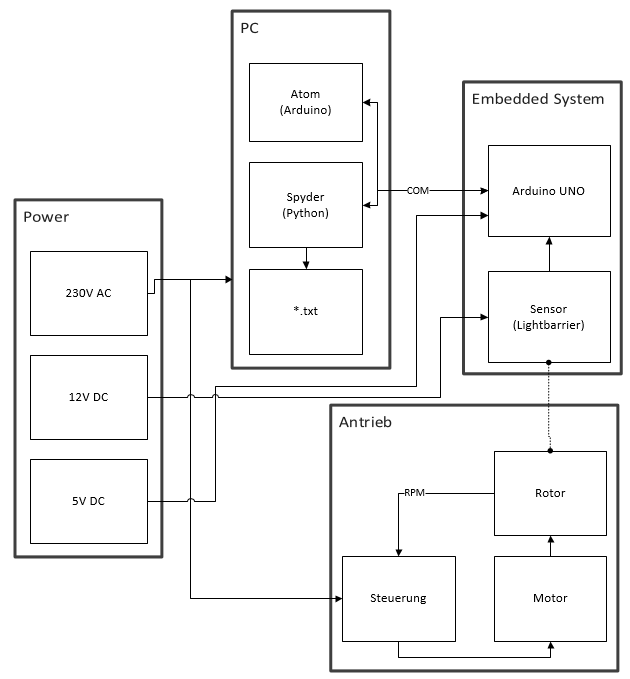
\includegraphics[width=\textwidth]{images/UebersichtVisio}
    \caption{Übersicht der Hardware}
    \label{fig:UebHardware}
\end{figure}
\subsection{Technische Daten der Lichtschranke}
\null\marg{Lichtschranke}
\begin{tabular}{ll}
    Hersteller & Panasonic\\
    Typ & Einweglichtschranke\\
    Modellnummer &  EX-21A-PN \\
    Schalttyp & Hell-EIN\\
    Reichweite & 1m\\
    Wiederholpräzision & max. 0.05 mm\\
    Ansprechzeit & max. 0.5 ms\\
    Spannung & 12 bis 24V DC $\pm$ 10\% \\
    Stromaufnahme & max. 10 mA
\end{tabular}
\\\null\\

Die kompletten Technischen Daten findet man in Anhang \ref{app:ex20}.\\

Bei der Auswahl der Lichtschranke wurde vor allem drauf geachtet, dass sie eine schnelle Reaktionszeit hat sowie eine gute Wiederholpräzision Weiter war es wichtig, dass sie Aktiv-Low ist, da nicht alle Arduinos auf ein HIGH-Signal einen Interrupt auslösen können.\\
\clearpage

\subsection{Arduino}
Als \marg{Arduino Uno} Embedded System wird ein Arduino Uno verwendet. Er wird wie in \ref{fig:ArdAns} gezeigt angeschlossen. Um die Ausgangsspannung der Lichtschranke von 12V auf das 5V-Level des Arduinos zu reduzieren wird ein Spannungsteiler verwendet. Die Berechnung dazu findet sich im Anhang \ref{app:berechnung}.\\


Für den Anschluss\marg{Anschluss} der Peripherie werden folgende Pins benötigt:\newline
\begin{tabular}{ll}
    \textbf{Pin} & \textbf{Bezeichnung}\\
    2 & Lichtschranke 1 (LB1)\\
    3 & Lichtschranke 2 (LB2)\\
\end{tabular}

\begin{figure}[ht]
    \centering
%    \missingfigure{Bild einfügen}
    \begin{subfigure}[c]{0.8\textwidth}       
        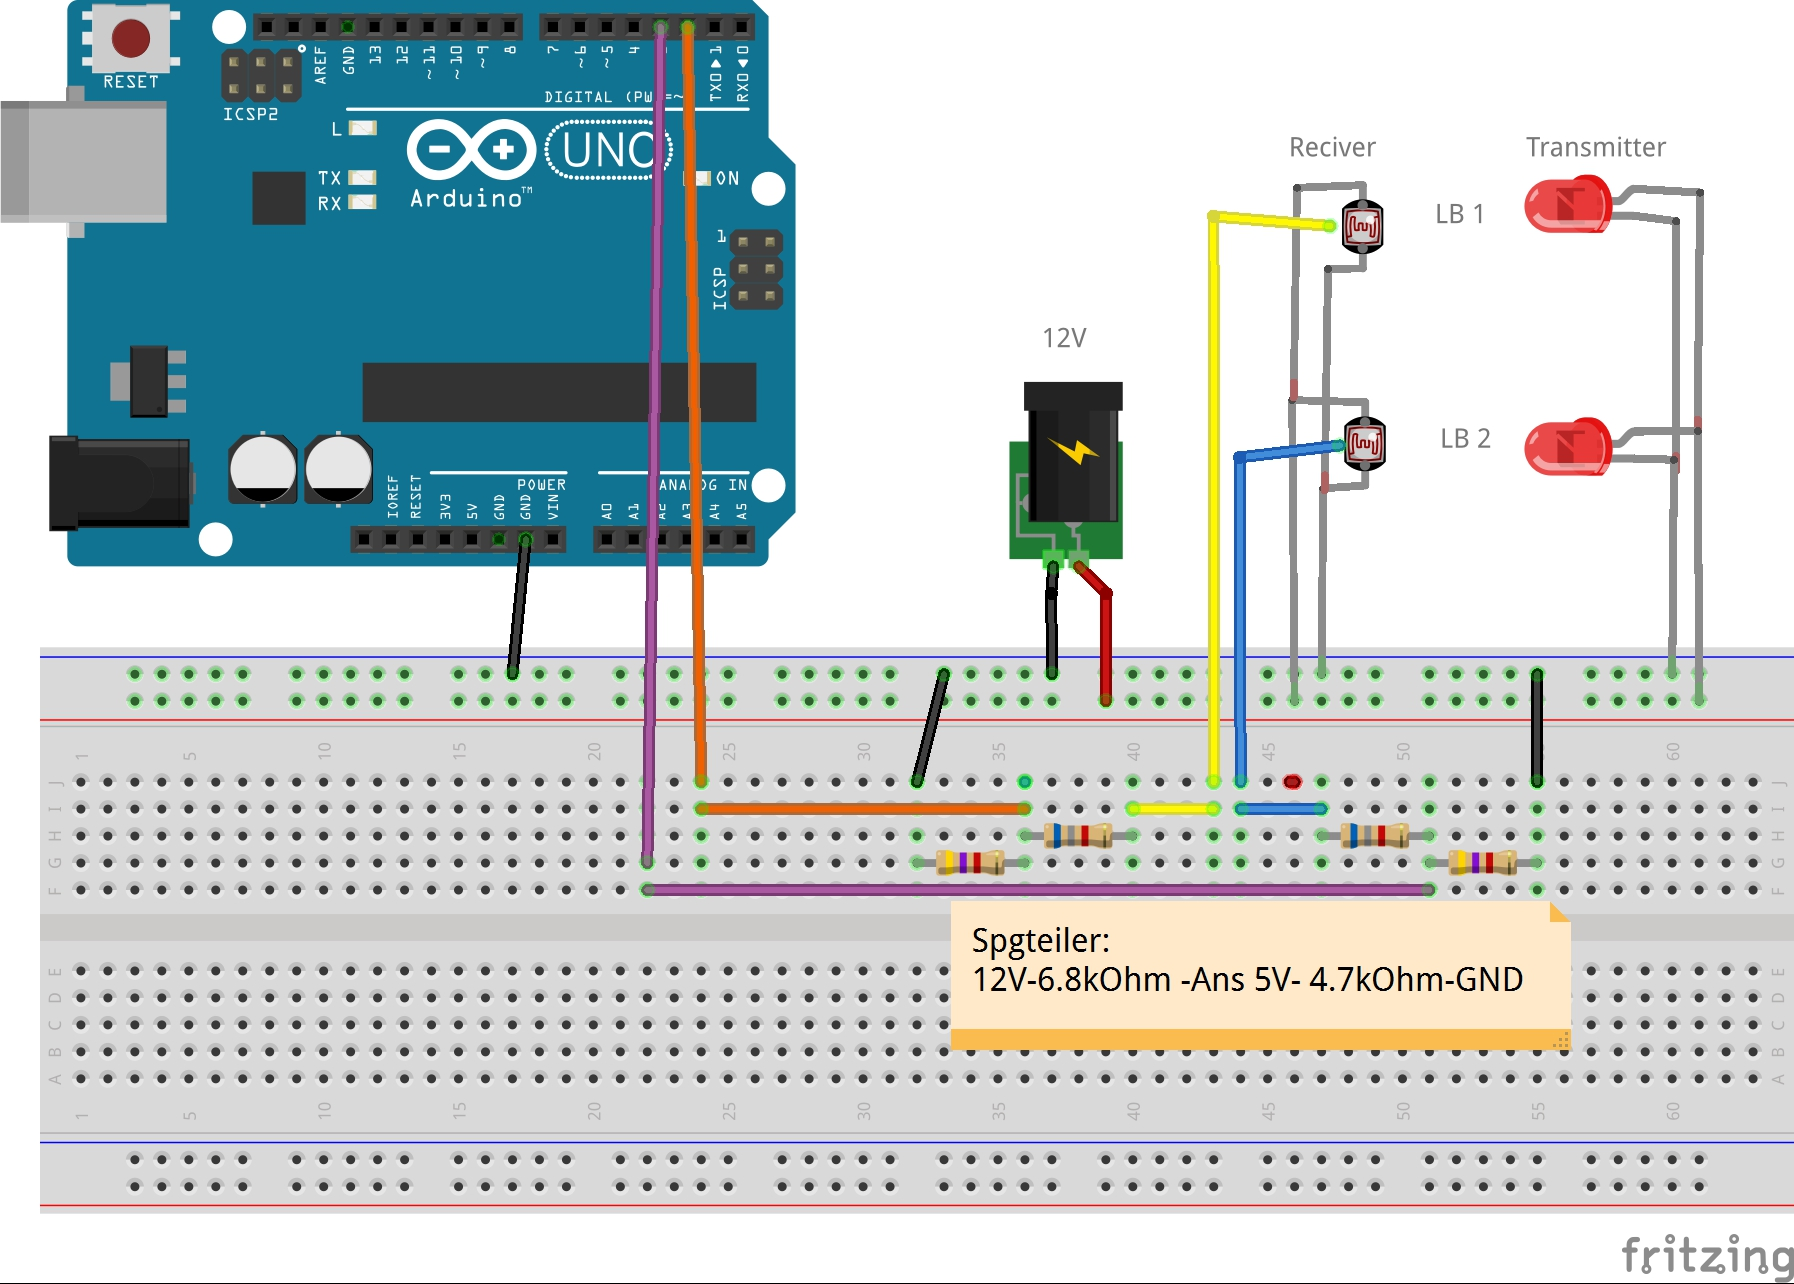
\includegraphics[width=\textwidth]{images/fritzing.jpg}
%        \subcaption{Übersicht}   
\null       
    \end{subfigure}
    
    \begin{subfigure}[c]{0.8\textwidth}
        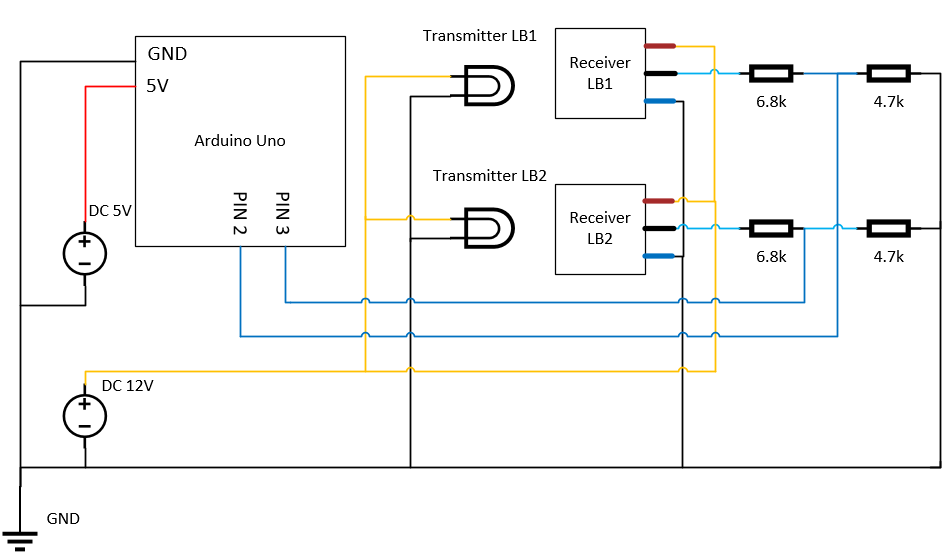
\includegraphics[width=\textwidth]{images/SchemaVisio.png}
%        \subcaption{Detail}
    \end{subfigure}
%   	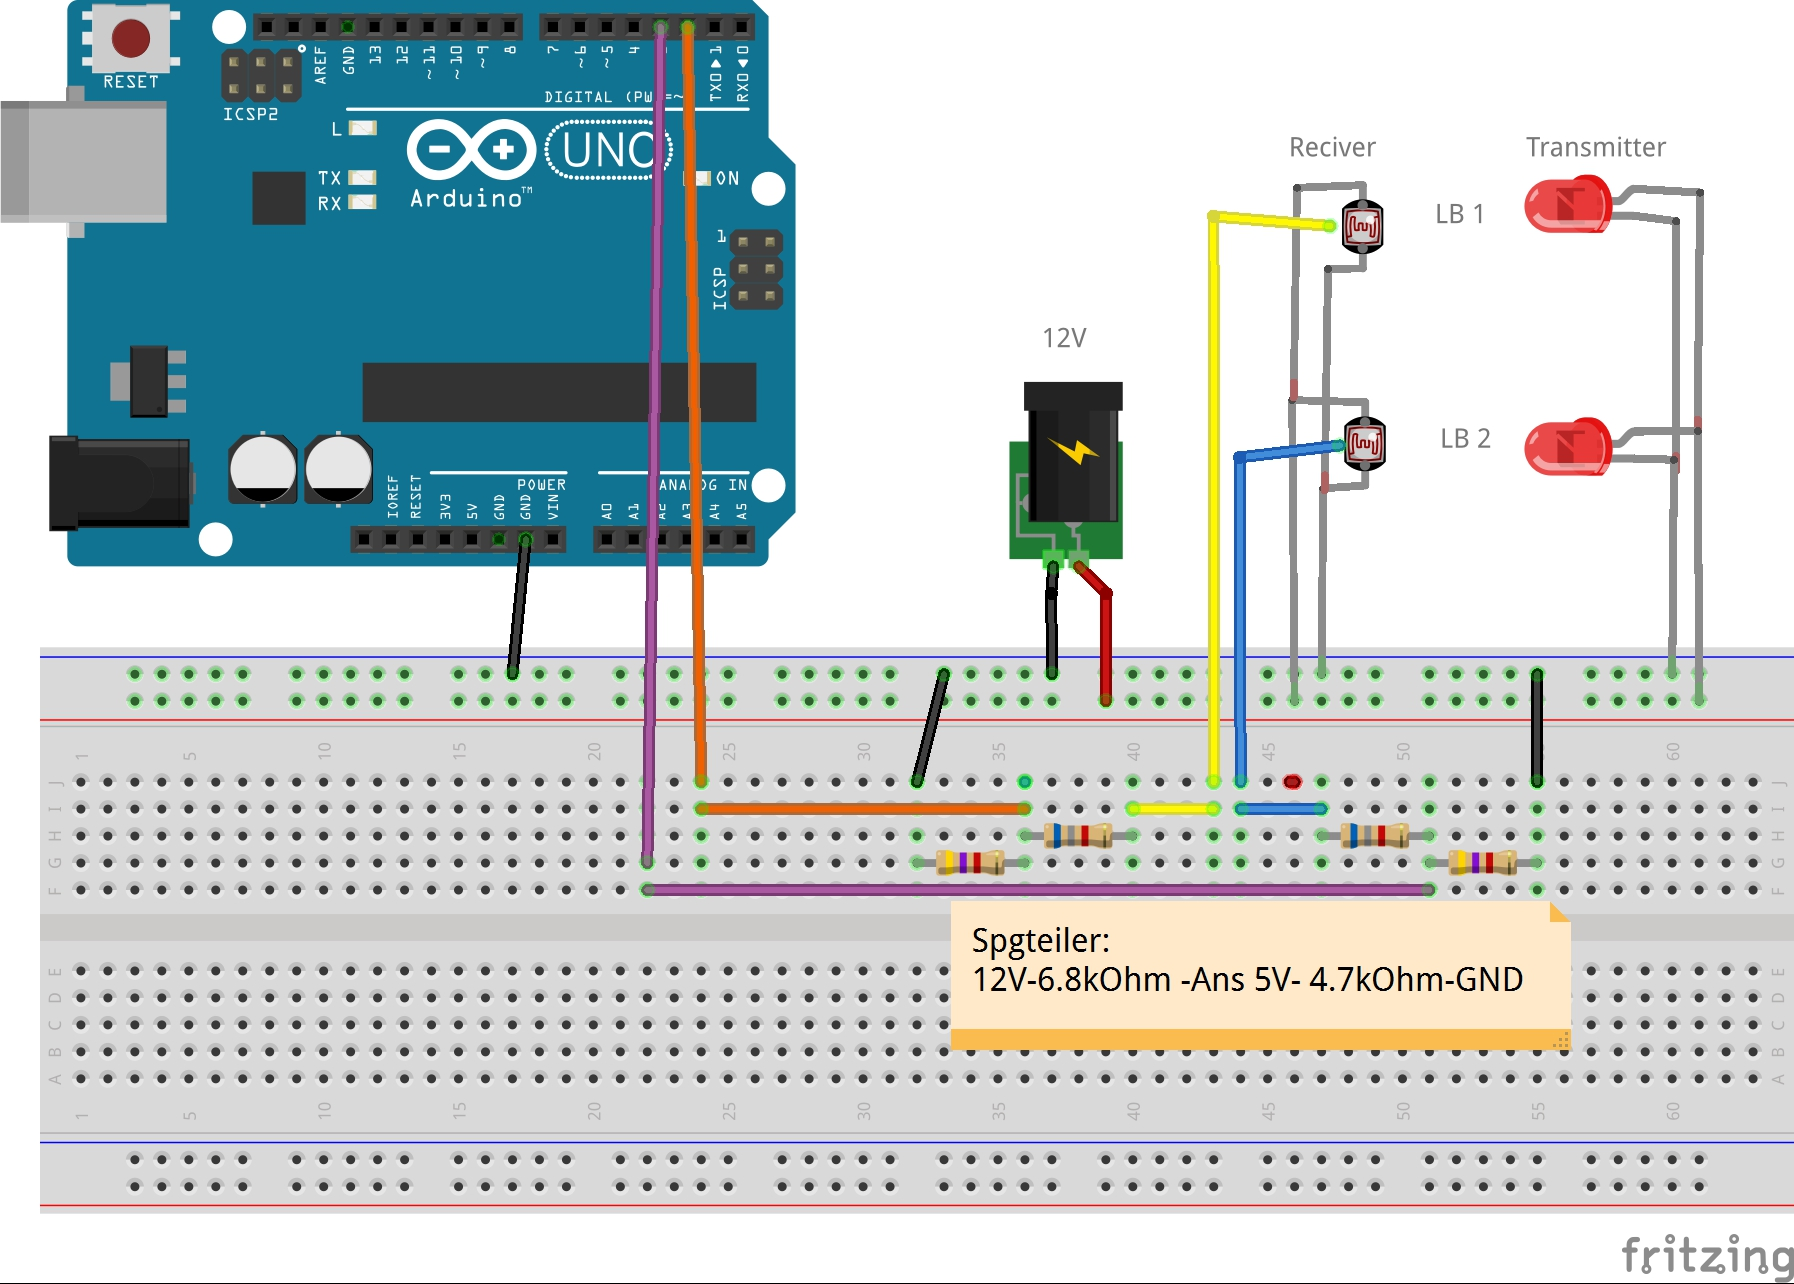
\includegraphics[width=\textwidth]{images/fritzing.jpg}
    \caption{Anschluss des Arduino Uno}
    \label{fig:ArdAns}
\end{figure}


    \clearpage\pagebreak
    \part{Software}
Softwareseitig wurde mit dem Plugin \href{https://platformio.org/platformio-ide}{PlatformIO} für Atom die Programmierung des Arduinos erstellt. Für Python wurde die \href{https://www.spyder-ide.org}{Spyder} IDE verwendet. Zur Versionierung wird \href{https://git-scm.com/}{Git} verwendet. Die Auswertung der Daten erfolgt mit Matlab und Excel.
\section{Programm}
Das Programm \textit{BWMvelocity.cpp} welches man in Anhang \ref{app:ardprog} findet, ermöglicht es mit Hilfe von Polling oder Interrupts die Unterbuchtszeiten der Lichtschranke zu erfassen und so auf Grund der Grösse des unterbrechenden Objekts oder auf Grund des Abstands der Lichtschranken auf die Geschwindigkeit zu schliessen.

\begin{equation}\label{eq:Geschwindigkeit}
    v = \frac{s}{\varDelta t}
\end{equation}
%\myequations{Berechnung der Geschwindigkeit}

\begin{table}[h] 
    \centering
    \begin{tabular}{cll}
        Parameter&Bemerkung&Einheit\\
        \hline
        $v$& Geschwindigkeit&$\left[\nicefrac{m}{s}\right]$\\
        $s$& Strecke&$\left[m\right]$\\
        $ \varDelta t$& Zeit&$\left[s\right]$\\
    \end{tabular}
    \caption{Übersicht der Parameter in \ref{eq:Geschwindigkeit}}
\end{table}

Ein Druchlauf \marg{Sensor-Signale} eines Objektes erzeugt dabei die in \ref{fig:ArdSigs} gezeigten Signale.
\begin{figure}[ht]
    \centering
    %    \missingfigure{Bild einfügen}
    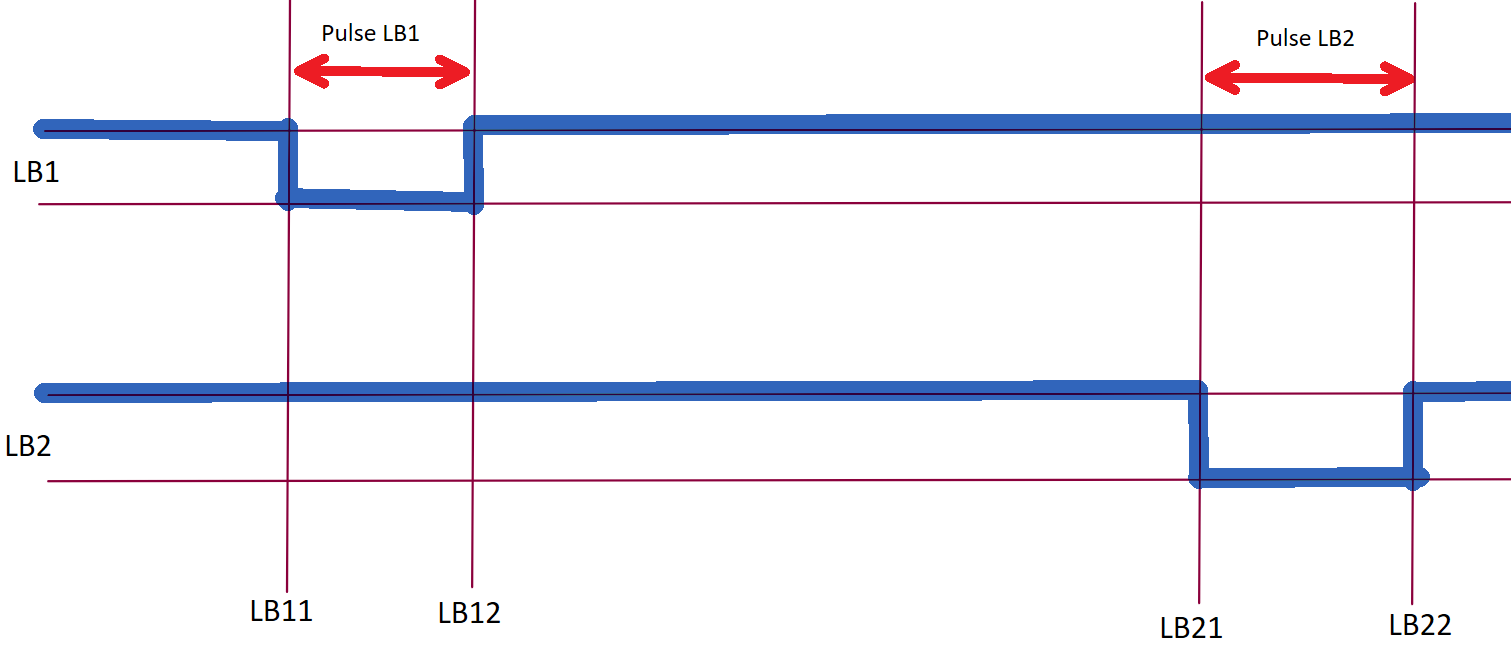
\includegraphics[width=\textwidth]{images/signals}
    \caption{Generierte Signale der Lichtschranke beim Durchflug eines Objekts abhängig der Zeit}
    \label{fig:ArdSigs}
\end{figure}


\clearpage
\subsection{Modi}
%\subsubsection{Preprocessor-Direktiven}
Mit\marg{Preprocessor} Hilfe der \#define Anweisung können drei verschiedene Modi ausgewählt werden. Dafür müssen die entsprechenden Befehle ein-kommentiert werden.\\

\begin{tabular}{L{0.3\linewidth} L{0.6\linewidth}}
    \#define MYDEBUG & Aktiviert den Debuggmodus und somit die \textit{DEBUG\_PRINT}-Funktionen.\\
    \#define MYLOG & Aktiviert den Datenloggingmodus und somit die \textit{LOG\_PRINT}-Funktionen.\\
    \#define USEINTERRUPT & Aktiviert den Interruptmodus und deaktiviert den Pollingmodus.\\
\end{tabular}\\

Der Debugg- und Logging-Modus ist nur für die Auswertung und/oder Fehlersuche über die serielle Schnittstelle relevant. Im Normalbetrieb (Polling- oder Interrupt-Modus) können sie auskommentiert bleiben.
\subsection{Globale Variabeln}
Es \marg{globale Variabeln} gibt folgende globale Variabeln:
\begin{itemize}
    \item const double sensordistance = 101.0*1000
    \item const double ballwidth = 72.0*1000
    \item unsigned long passingtime[4]
    \item double velocitykmh[4]
    \item int countingvar
\end{itemize}

\textit{sensordistance} und \textit{ballwidth} beschreiben die geometrischen Randbedingungen in $\mu m$.\\
\textit{passingtime} beinhaltet die Zeitstempel in $\mu s$ und \textit{velocitykmh} beinhaltet die gemessenen Geschwindigkeiten in $\nicefrac{km}{h}$.\\
Bei \textit{countigvar} handelt es sich um eine Lauf-variabel zur Indexierung der SerialPrint-Ausgaben.


\subsection{Hilfsfunktionen}
\subsubsection{calculate\_velocity\_ms()}\label{subsubsec:calcvel}
\begin{center}
    Geschwindigkeit [$\nicefrac{m}{s}$] = calculate\_velocity\_ms( Zeit [$\mu S$], Distanz [$\mu m$])
\end{center}

Die Funktion \textit{double calculate\_velocity\_ms(unsigned long passingduration,double distance)} übernimmt eine Zeitdauer in $\mu S$ und eine Distanz in $\mu m$.
Sie giebt eine Geschwindigkeit mit Hilfe der \ref{eq:Geschwindigkeit} in $\nicefrac{m}{s}$ zurück vom Typ double.\\


\subsubsection{printlog()}
Wenn der Datenlogging-Modus aktiv ist printet die Funktion in die serielle Schnittstelle.\\
Im Pollingmodus:\\
\begin{tabular}{llll}
    Iteration&Bezeichnung& Puls LB1 & Puls LB2\\
\end{tabular}

Im Interruptmodus:\\
\begin{tabular}{llllll}
    Iteration&Bezeichnung& Int. LB1 & Int. LB2& Int. LB11 - LB21& Int. LB12 - LB22\\
\end{tabular}\\

\clearpage
\subsection{Polling-Modus}\label{subsec:polling}
Im \marg{Polling} Polling-Modus wird mit der Funktion \textit{\href{https://www.arduino.cc/reference/en/language/functions/advanced-io/pulsein/}{pulseIn(pin, value, timeout)}} die Länge des Unterbruches in $\mu S$ angegegeben. Die minimale dedektierbare Pulslänge ist dabei 10 $\mu S$.
Es werden folgende Zeiten erfasst und im Array \textit{passingtime} abgelegt:
\begin{center}
    \begin{tabular}{cll}
        \textbf{Index}&\textbf{Zeit [$\mu S$]} & \textbf{relevante Distanz} \\
        0&Pulse LB1 & Objektgrösse\\
        1&Pulse LB2 & Objektgrösse\\
    \end{tabular}\\
\end{center}
Die Werte im Index 2 und 3 sind im Pollingmodus immer 0.\\

Mit der Funktion \textit{calculate\_velocity\_ms()}(Abschnitt \ref{subsubsec:calcvel}) kann die Geschwindigkeit in $\nicefrac{m}{s}$ berechnet werden. Danach wird das Resultat mit dem Faktor 3.6 multipliziert und im Array \textit{velocitykmh} abgelegt.\\

Die Werte im Index 2 und 3 sind im Pollingmodus immer 0.\\


\subsection{Interrupt-Modus} \label{subsec:interrupt}
Im \marg{Interrupt}Interrupt-Modus wird bei jedem Flankenwechsel ein Interrupt ausgelöst und ein Zeitstempel in $\mu S$ gespeichert.\\
\textbf{Beim Arduino UNO müssen die Lichtschranken dafür zwingend auf Pin 2 und 3 angeschlossen sein. Weiter muss zuerst die Lichtschranke 1 danach Lichtschranke 2 ausgelöst werden.} Dies liegt daran, dass beim Durchlauf von LB22 das Flag \textit{LBinterrupted} gesetzt wird. Werden die Lichtschranken vertauscht, erfolgt die Auslösung an der Position LB12 (vgl. \ref{fig:ArdSigs})\\
Dies ergibt gesamt 4 Messwerte für LB11, LB12, LB21 und LB22 wie in \ref{fig:ArdSigs} gezeigt. Diese werden im Array \textit{passingtime} gespeichert.\\

Das Array \textit{passingtime} beinhaltet also im Interruptmodus die folgenden Einträge:
\begin{center}
    \begin{tabular}{cl}
        \textbf{Index}&\textbf{Zeit [$\mu S$]} \\
        0&LB11 \\
        1&LB12 \\
        2&LB21 \\
        3&LB22 \\
    \end{tabular}\\
\end{center}
Mit der Funktion \textit{calculate\_velocity\_ms()}(\ref{subsubsec:calcvel}) kann die Geschwindigkeit in $\nicefrac{m}{s}$ berechnet werden. Danach wird das Resultat mit dem Faktor 3.6 multipliziert und im Array \textit{velocitykmh} abgelegt.
\begin{center}
    \begin{tabular}{cll}
        \textbf{Index}&\textbf{Zeit [$\mu S$]} & \textbf{relevante Distanz [$\mu m$]} \\
        0&LB12 - LB11 & Objektgrösse\\
        1&LB22 - LB21 & Objektgrösse\\
        2&LB21 - LB11 & Sensorabstand\\
        3&LB22 - LB12 & Sensorabstand\\
    \end{tabular}\\
\end{center}
\subsubsection{Hilfsfunktionen}
Der Interruptmodus benötigt noch weitere Hilfsfunktionen, nämlich die Interrupt-Service-Routine. Weiter wird noch das Flag \marg{Interrupt-Flag} \textit{LBinterrupted} benötigt, welches auf True wechselt, sobald das Objekt den Punkt LB22 durchlaufen hat.\\


\paragraph{ISRLB1()}
Diese Funktion ist die Interrupt-Service-Routine für die Lichtschranke LB1. Sie erkennt den Signalwechsel und schreibt den aktuellen Zeitstempel LB11 oder LB12 je nach dem ob das Signal HIGH oder LOW ist. Weiter wird das Flag \textit{LBinterrupted} auf False gesetzt.\\


\paragraph{ISRLB2()}
Diese Funktion ist die Interrupt-Service-Routine für die Lichtschranke LB1. Sie erkennt den Signalwechsel und schreibt den aktuellen Zeitstempel LB11 oder LB12 je nach dem ob das Signal HIGH oder LOW ist. Bei LB21 wird das Flag \textit{LBinterrupted} auf False gesetzt. Bei LB22 auf True.\\


%
%Der \marg{Funktionen} Code besitzt folgende Funktionen:
%\begin{itemize}
%    \item void setup()
%    \item void loop()
%    \item double calculate\_velocity\_ms(unsigned long passingduration,double distance)
%    \item void printlog(double speedinkmh[4])
%    \item void ISRLB1()
%    \item void ISRLB2()
%\end{itemize}
%
%
%Das Array \textit{passingtime} beinhaltet die folgenden Einträge:\\
%\begin{tabular}{lll}
%    \textbf{Index}&\textbf{Zeit} & \textbf{Distanz} \\
%    0&LB12 - LB11 & Ballgrösse\\
%    1&LB22 - LB21 & Ballgrösse\\
%    2&LB21 - LB11 & Sensorabstand\\
%    3&B22 - LB12 & Sensorabstand\\
%\end{tabular}\\
%
%Das Array \textit{velocitykmh} beinhaltet die berechneten Geschwindigkeit korresponidrenden zu den Zeiten und Distanzen aus dem passingtime-Array.\\
%Im Pollingmodus sind die Werte bei  Index 2 und 3 jeweils 0.
\subsection{Hauptfunktionen}
\subsubsection{setup()}
Die \textit{setup()}-Funktion läuft nur ein mal beim Einschalten oder dem Reset des Arduinos durch. Sie initialisiert die serielle Kommunikation und erstellt die Interrupt-Zuweisung der Pins im Interrupt-Modus. Ausserdem erstellt sie die erste Zeile des Log-Files im Logging-Modus.\\


\subsubsection{loop()}
Die \textit{loop()}-Funktion wird nach der \textit{setup()}-Funktion dauernd ausgeführt. In ihr läuft das Hauptprogramm. Je nach aktivem Modus entweder im Polling- oder im Interrupt-Modus.

\clearpage

\section{Python}
Das Pythonskript aus Anhang \ref{app:python} dient dazu, die gesendeten Daten über den Serialport auszulesen und in einem .txt File abzuspeichern. Dies erleichtert die Datenanalyse mit Excel oder Matlab. Eine direkte Auswertung in Phyton wäre ebenfalls möglich.\\


\subsection{Randbedingungen}
Die Baudrate im Python-Sktipt (Zeile 29) muss die selbe sein wie im Arduino-Code angegeben.\\
Der COM-Port sollte unter Windows automatisch gefunden werden. Ist dies nicht der Fall müssen die Zeilen 31 bis 38 angepasst werden. Das Argument \textit{serial\_port} kann dabei einfach mit dem gewünschten Port ersetzt werden.\\


\subsection{Messdaten}
Der Name des Ausgabefiles kann in Zeile 48 beliebig angepasst werden.\\


\subsection{Ablauf}
Wird das Skript gestartet erstellt es ein *.txt-File und schreibt eine Kopfzeile.
Danach wird alles, was über den gewählten Serialport empfangen wird in dieses .txt-File gespeichert.\\
Sobald ein \textit{KeyboardInterrupt} erzeugt wird, beispielsweise mit Ctrl + C oder dem Abbruch-Knopf wird das File gespeichert und das Skript beendet.
    \clearpage\pagebreak
    \part{Versuch}
\section{Aufbau}
Der Versuchsaufbau wurde im Zimmer 2.001b mit einem Servomotor aus den Praktikas durchgeführt. Er kann zwischen -2500 bis +2500 $\nicefrac{U}{min}$ betrieben werden und im \textit{Syncronisation Mode} auf 1 $\nicefrac{U}{min}$ genau eingestellt werden. Im \textit{Normal Mode} liegt die Schrittweite bei 10 $\nicefrac{U}{min}$.

\begin{figure}[ht]
    \centering
    %    \missingfigure{Bild einfügen}    
    \begin{subfigure}[c]{0.8\textwidth}       
        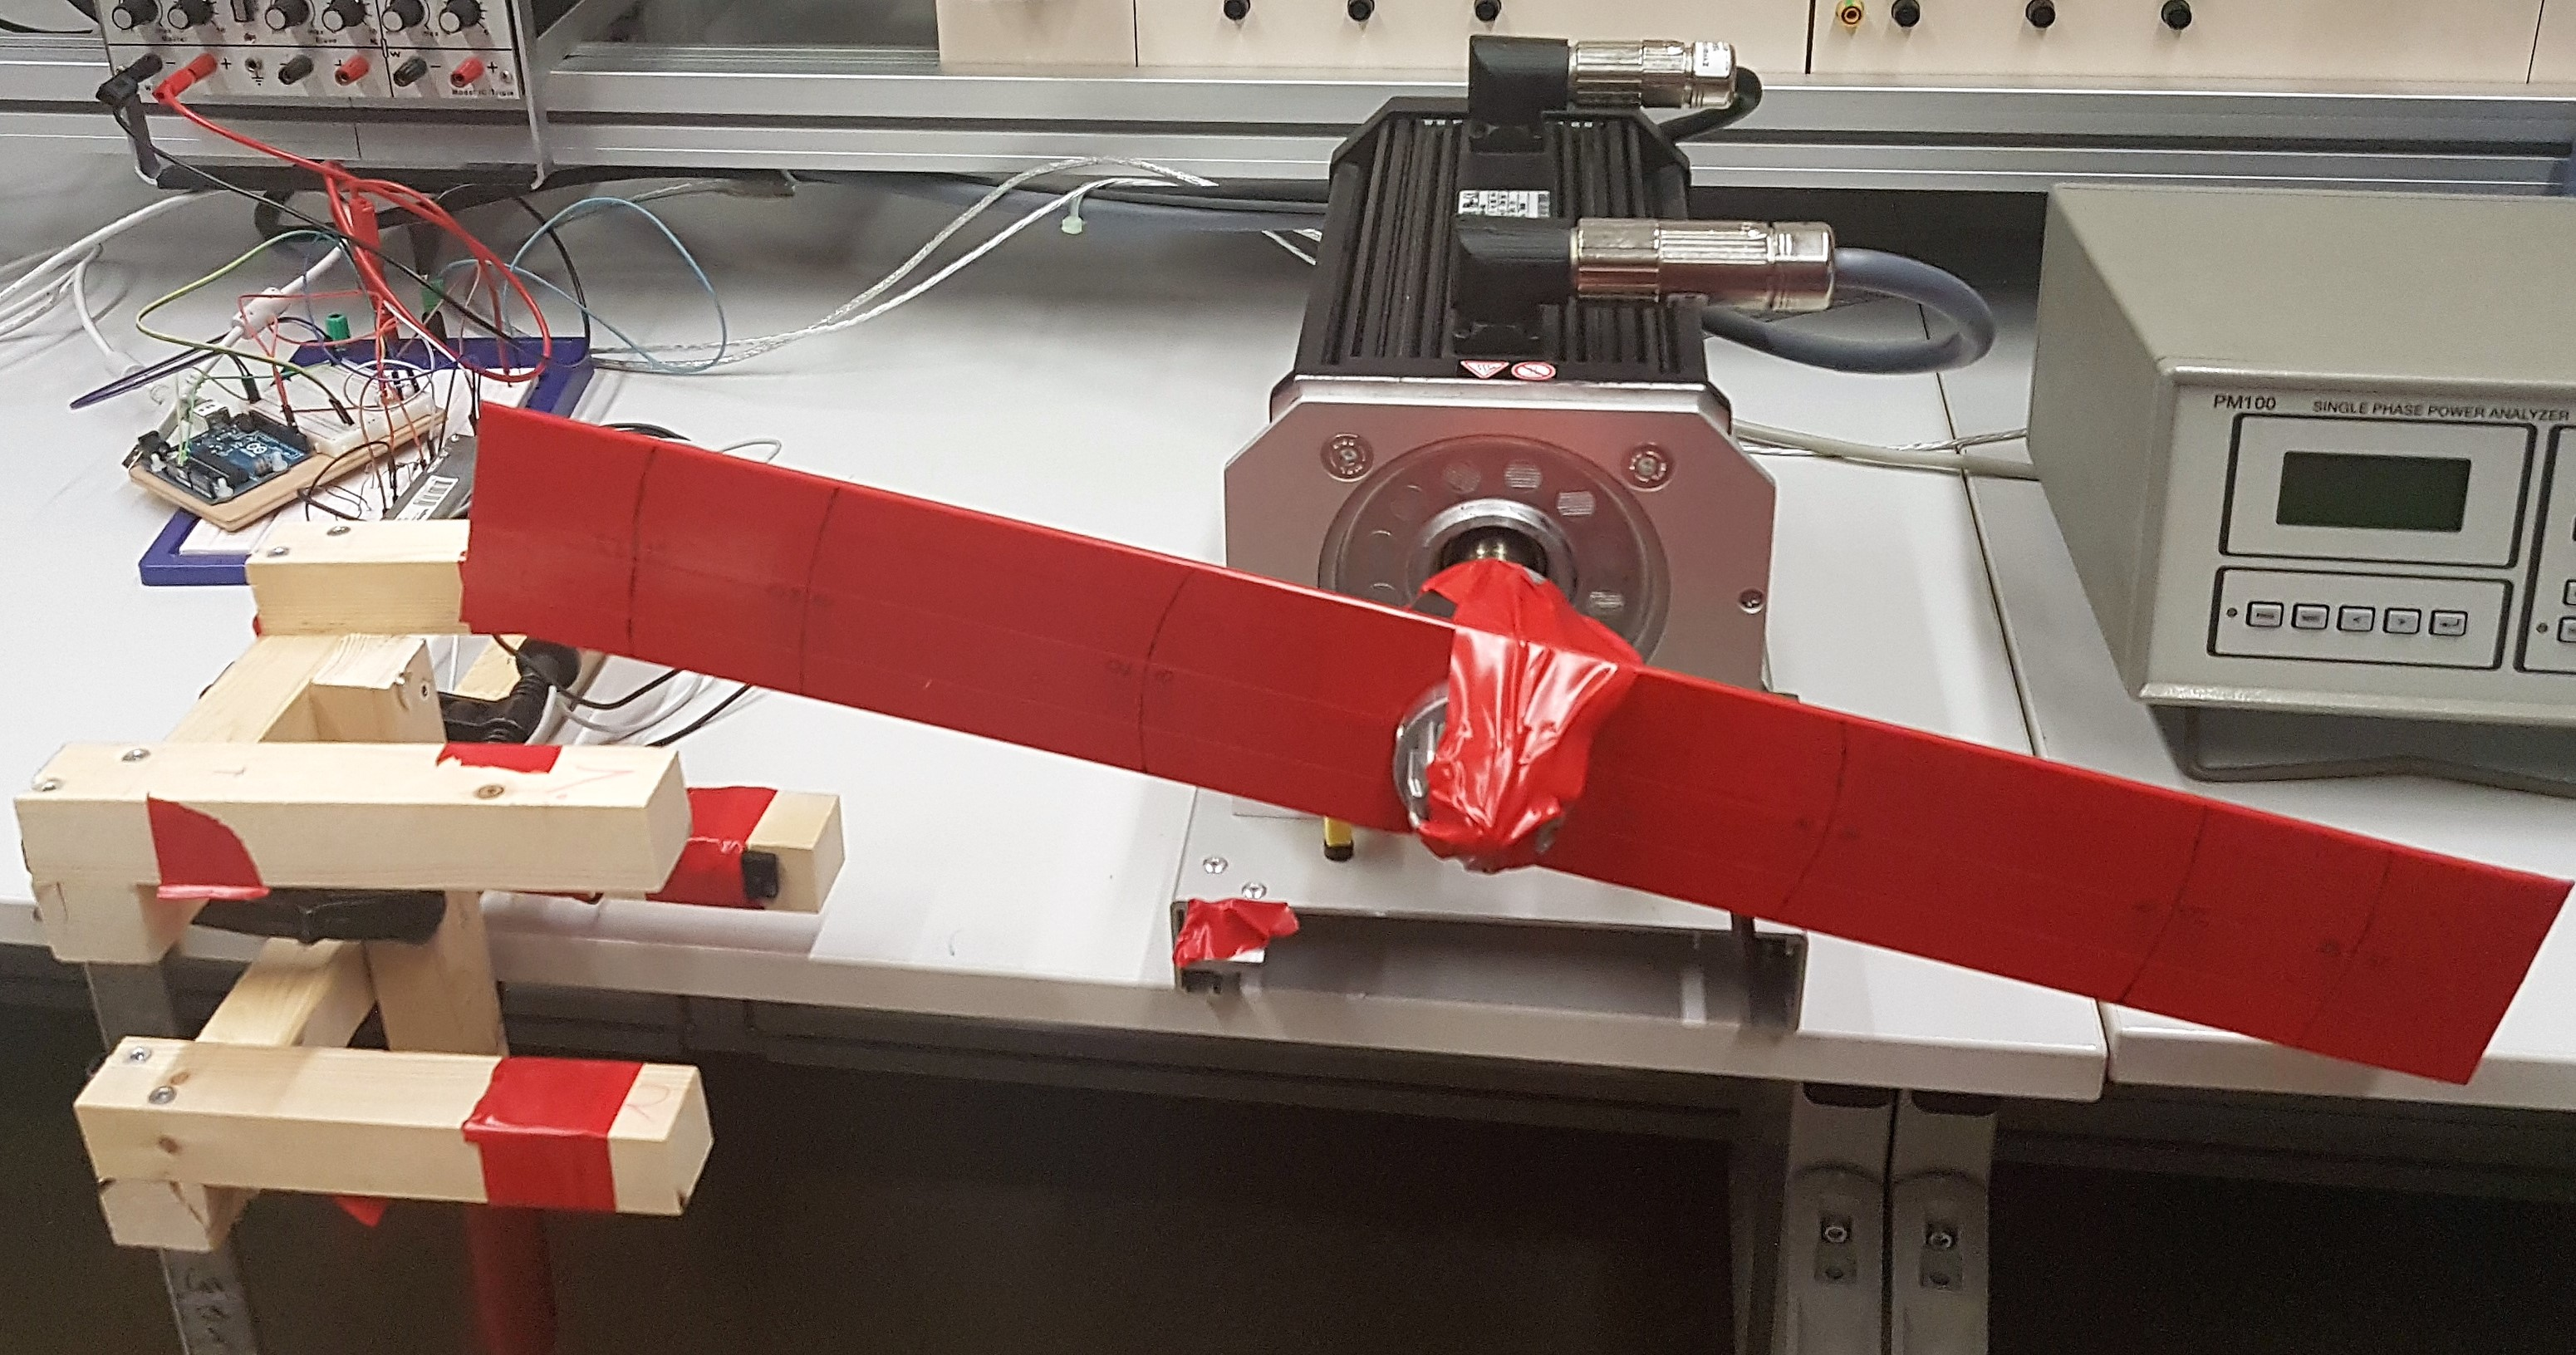
\includegraphics[width=\textwidth]{images/Aufbau.jpg}
        \subcaption{Übersicht}          
    \end{subfigure}

    \begin{subfigure}[c]{0.8\textwidth}
        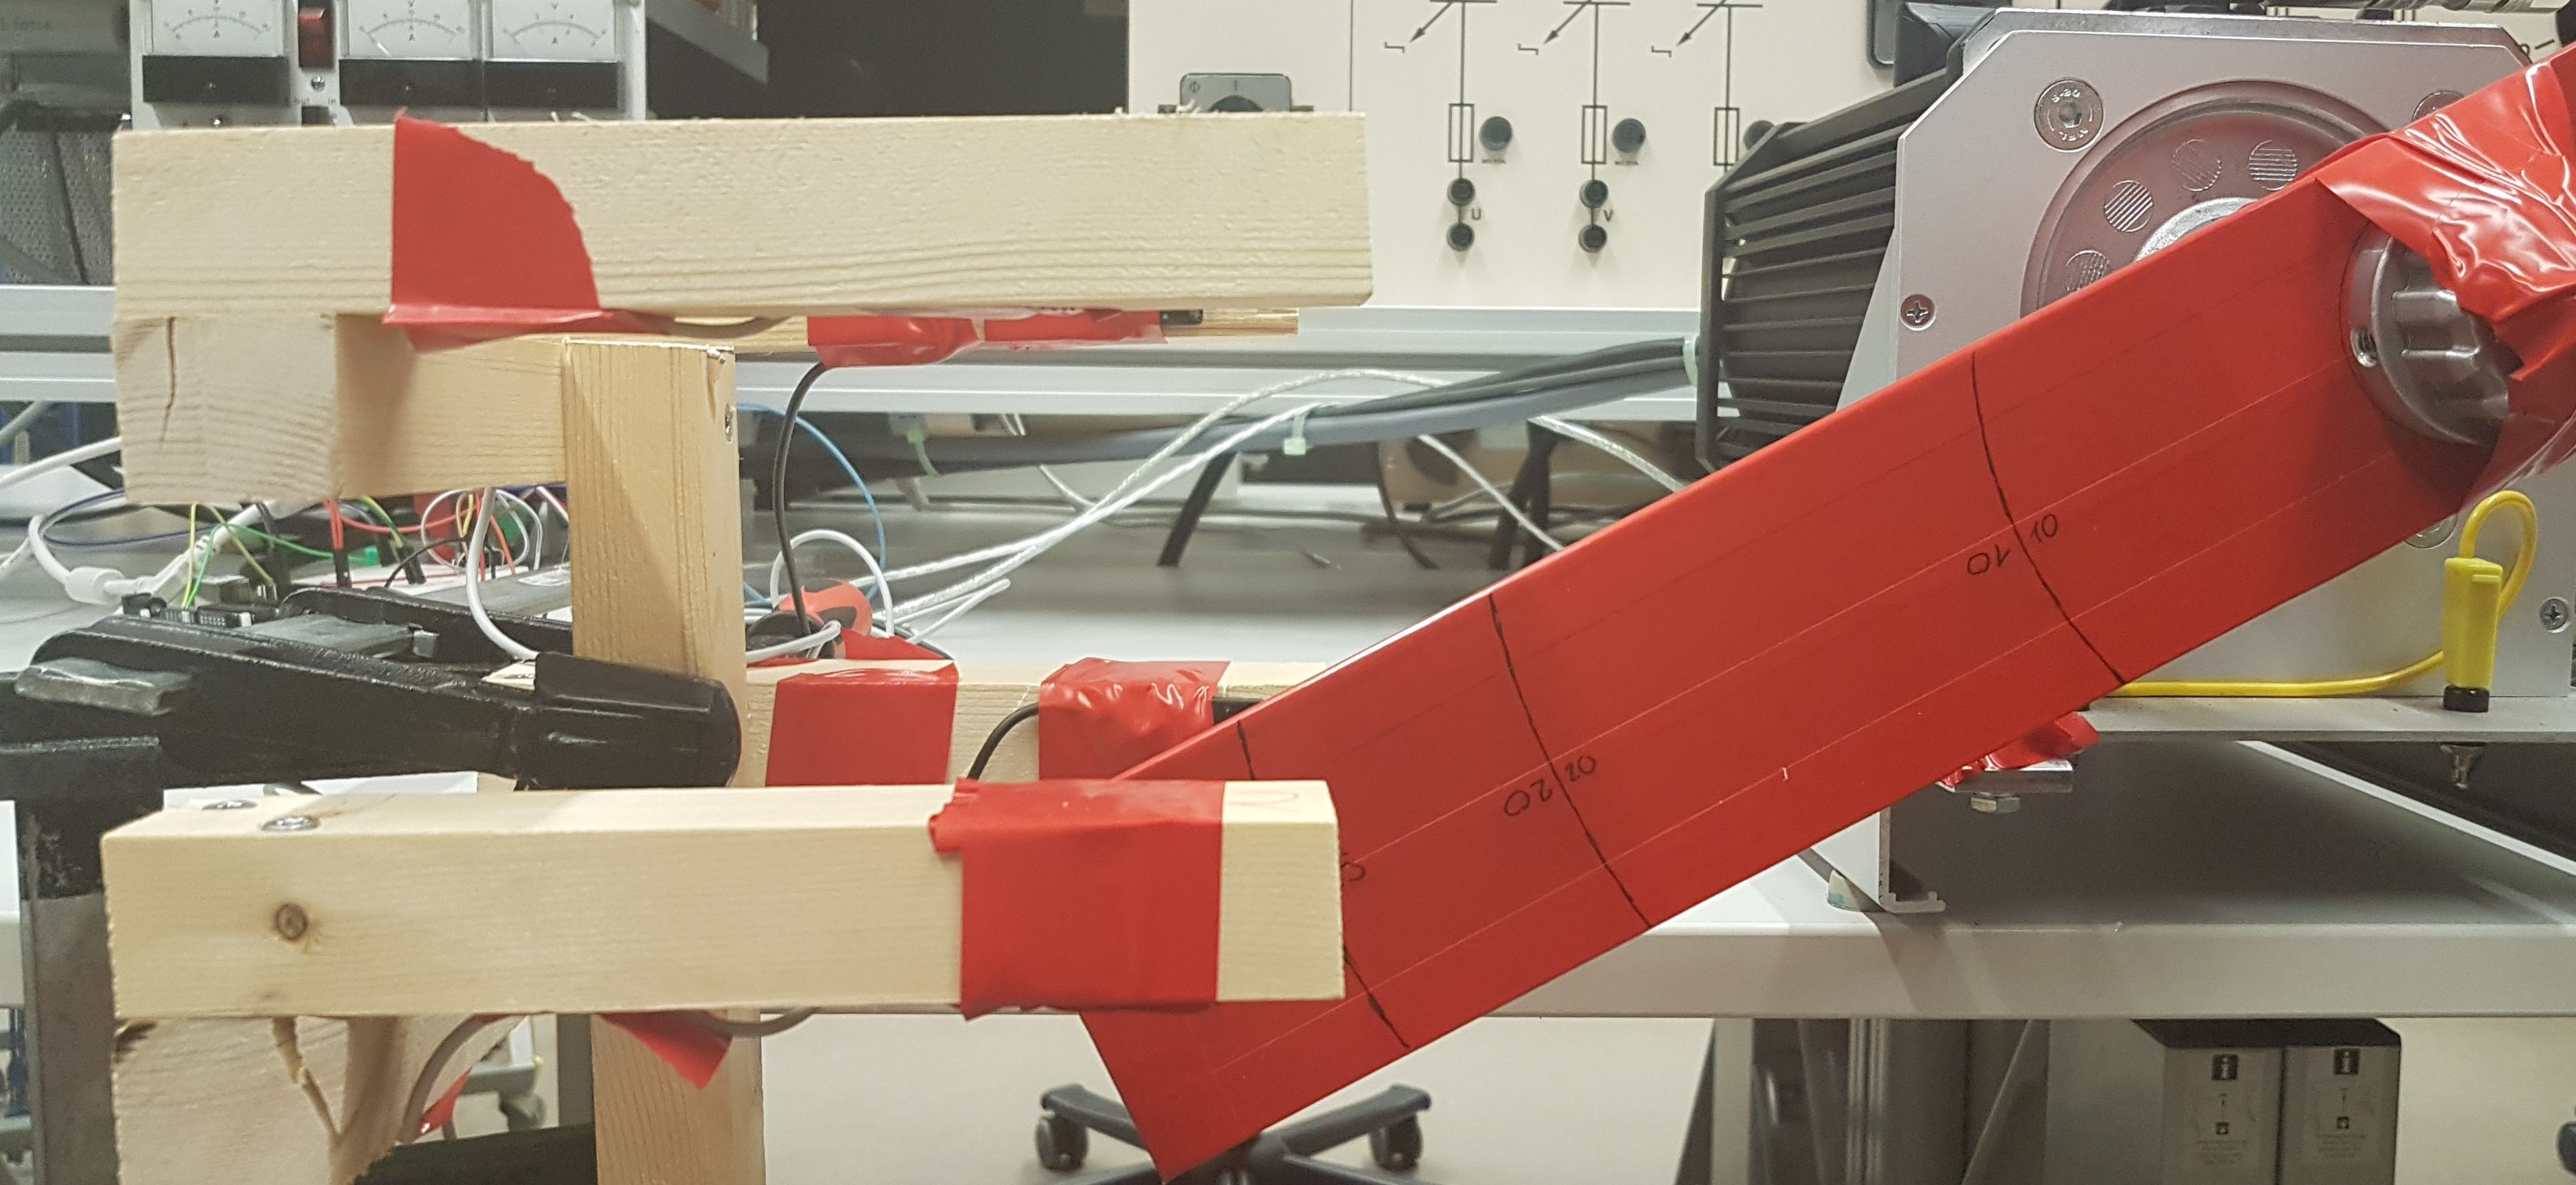
\includegraphics[width=\textwidth]{images/AufbauDetail.jpg}
        \subcaption{Detail}
    \end{subfigure}
    \caption{Versuchsaufbau}\label{fig:Aufbau}   
\end{figure}

Die Lichtschranken wurden mit Hilfe einer Holzkonstruktion montiert.\\
Sie haben einen Abstand von 100mm.\\
Der \marg{Rotor} Rotor ist 72mm breit und somit die Dimension eines Unihockeyballs.\\

Bei einem Durchmesser von 50cm ergibt sich mit 2000 $\nicefrac{U}{min}$ eine Umfangsgeschwindigkeit von 188.5 $\nicefrac{km}{h}$ wie man dem Anhang \ref{app:berechnung} entnehmen kann.
    \clearpage\pagebreak
    \section{Auswertung}
Mit dem Aufbau ist es möglich Geschwindigkeiten von über 200 $\nicefrac{km}{h}$ zu erzeugen.

\begin{figure}[ht]
    \centering
    %    \missingfigure{Bild einfügen}
    \includegraphics[width=\textwidth]{images/auswertungSpeedUeb.png}
    \caption{Vergleich unterschiedliche Geschwindigkeiten}
    \label{fig:AuswertungSpeed}
\end{figure}

In \ref{fig:AuswertungSpeed} werden die verschiedenen gemessenen Geschwindigkeit abhängig von der Drehzahl dargestellt.
Erwartet sind folgende Geschwindigkeiten:
\begin{center}
    \begin{tabular}{rr}
        \textbf{RPM}&\textbf{Geschwindigkeit $\left[\nicefrac{km}{h}\right]$}\\ \hline
        100&9.4\\
        500&47.1\\
        750&70.7\\
        1000&94.2\\
        1250&117.8\\
        1500&141.4\\
        1750&164.9\\
        2000&188.5\\
    \end{tabular}
\end{center}
 Die Präzision nimmt mit höherer Geschwindigkeit immer weiter ab, während die Genauigkeit etwa gleich bleibt (vgl. \ref{fig:AuswertungSpeed}, \ref{fig:GenauPraz}). 
% Dieses Verhalten zeigt auch \ref{fig:AuswertungZeitfehler}.

\begin{figure}[ht]
    \centering
    %    \missingfigure{Bild einfügen}
    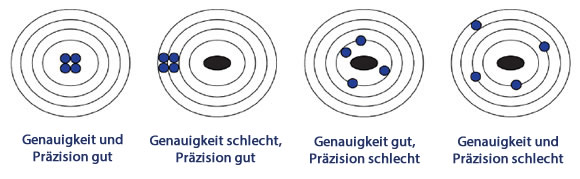
\includegraphics[width=0.7\textwidth]{images/testingtips}
    \caption{Genauigkeit und Präzision}
    \label{fig:GenauPraz}
\end{figure}
\clearpage

In \ref{fig:AuswertungInt} \marg{Vergleich Polling - Interrupt} werden die verschiedene Implementationsmethoden verglichen.\\

Die Daten für Puls LS1 und Puls LS2 wurden durch Polling gewonnen während die restlichen durch Interrupts generiert wurden. Detailliertere Grafiken dazu finden sich in Anhang \ref{app:Auswertung}.
\begin{figure}[ht]
    \centering
%    \missingfigure{Bild einfügen}
    	\includegraphics[width=\textwidth]{images/auswertungInt.png}
    \caption{Vergleich Interrupt und Polling bei 1000 RPM (94.2 $\nicefrac{km}{h}$)}
    \label{fig:AuswertungInt}
\end{figure}


Bei 2000 RPM wurden in beiden Modi jeweils 500 Sample aufgezeichnet und ausgewertet. Dabei wurde eine Präzision von unter 2\% und eine Genauigkeit von unter 5\% erreicht.\\
Die Histogramme aus \ref{fig:Hist} wurde mit Hilfe eines Matlabskripts (Anhang \ref{app:matlab}) erstellt und ausgewertet.\\
% (\href{https://ch.mathworks.com/help/stats/histfit.html}{histfit}). Möglich ist auch eine andere Verteilung. Dies muss genauer untersucht werden.

Berechnung Genauigkeit\marg{Genauigkeit} [\%]:
\[ \frac{|Sollgeschwindigkeit - Mittelwert\;der \; Samples|}{Sollgeschwindigkeit}\cdot 100 \]

Berechnung Präzision \marg{Präzision} [\%]:
\[ \frac{Standardabweichung\;der \; Samples}{Mittelwert\;der \; Samples}\cdot 100 \]

\begin{center}
    \begin{tabular}{lccc}
        \textbf{Mode} & \textbf{Messung} & \textbf{Genauigkeit [\%]} & \textbf{Präzision [\%]} \\ \hline
        Polling       &       LB1        & 4.9                     &  1.9                    \\
        &       LB2        & 3.8                     &  1.6                    \\
        Interrupt     &   LB11 - LB12    & 3.5                     &  1.8                    \\
        &   LB21 - LB22    & 2.4                     &  1.5                    \\
        &   LB11 - LB21    & 3.4                     &  1.2                    \\
        &   LB12 - LB22    & 2.6                     &  1.2 \\
    \end{tabular}
\end{center}

\clearpage

\begin{figure}[H]
    \centering
    %    \missingfigure{Bild einfügen}
    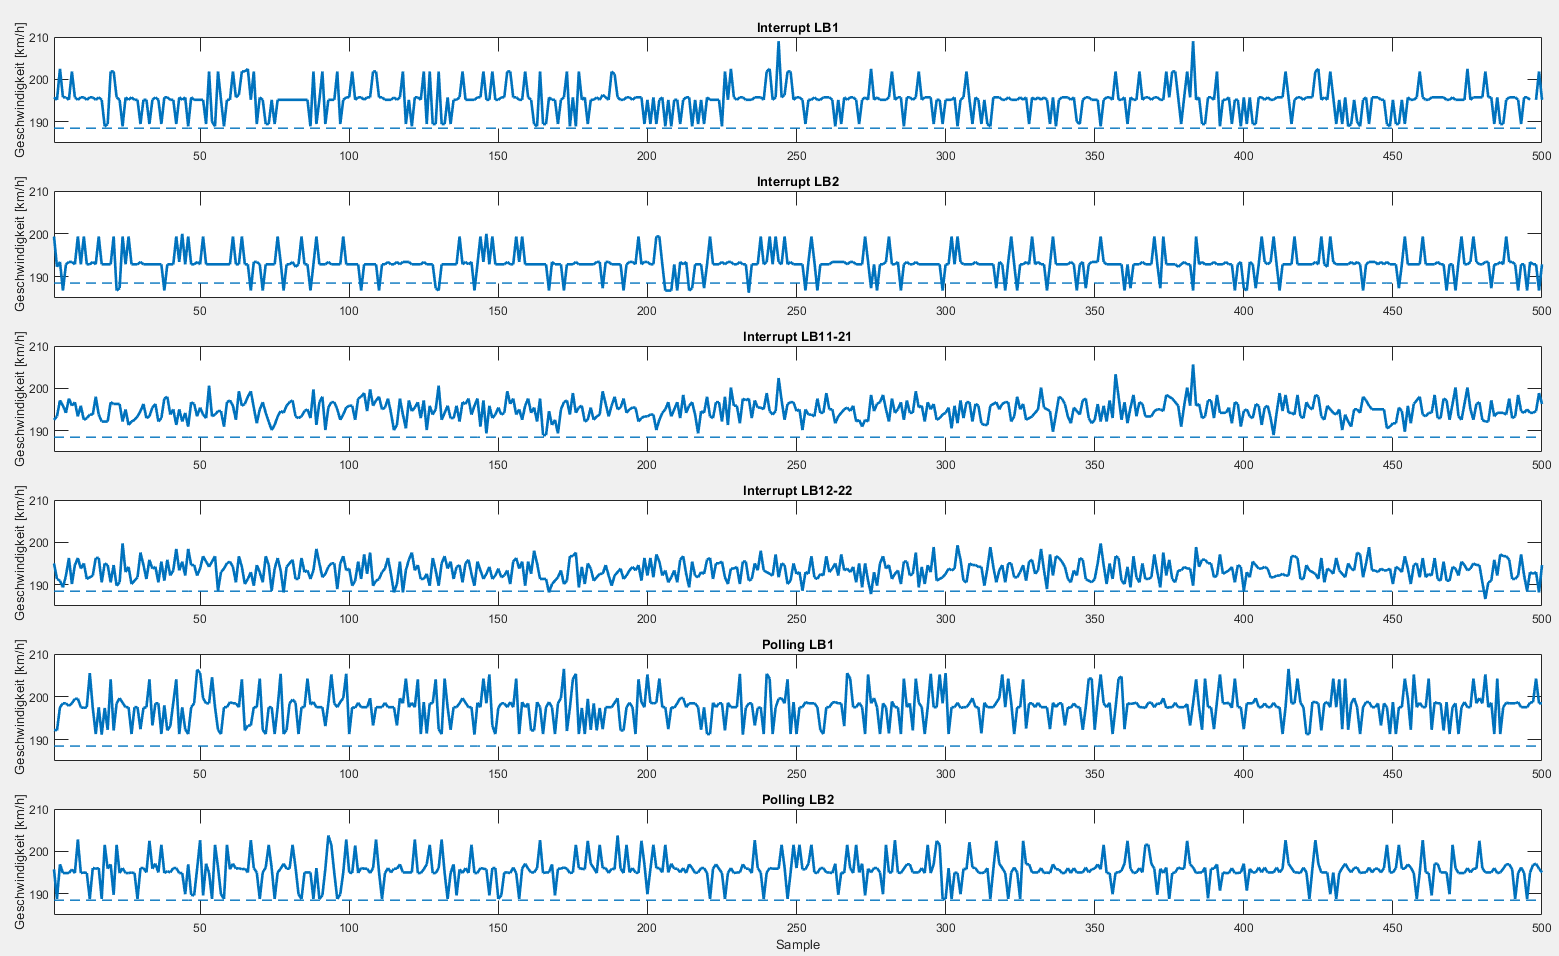
\includegraphics[width=\textwidth]{images/sig2000.png}
    \caption{Gemessene Werte bei 2000 RPM}
    \label{fig:sig2000}
\end{figure}
\begin{figure}[H]
    \centering
    %    \missingfigure{Bild einfügen}
    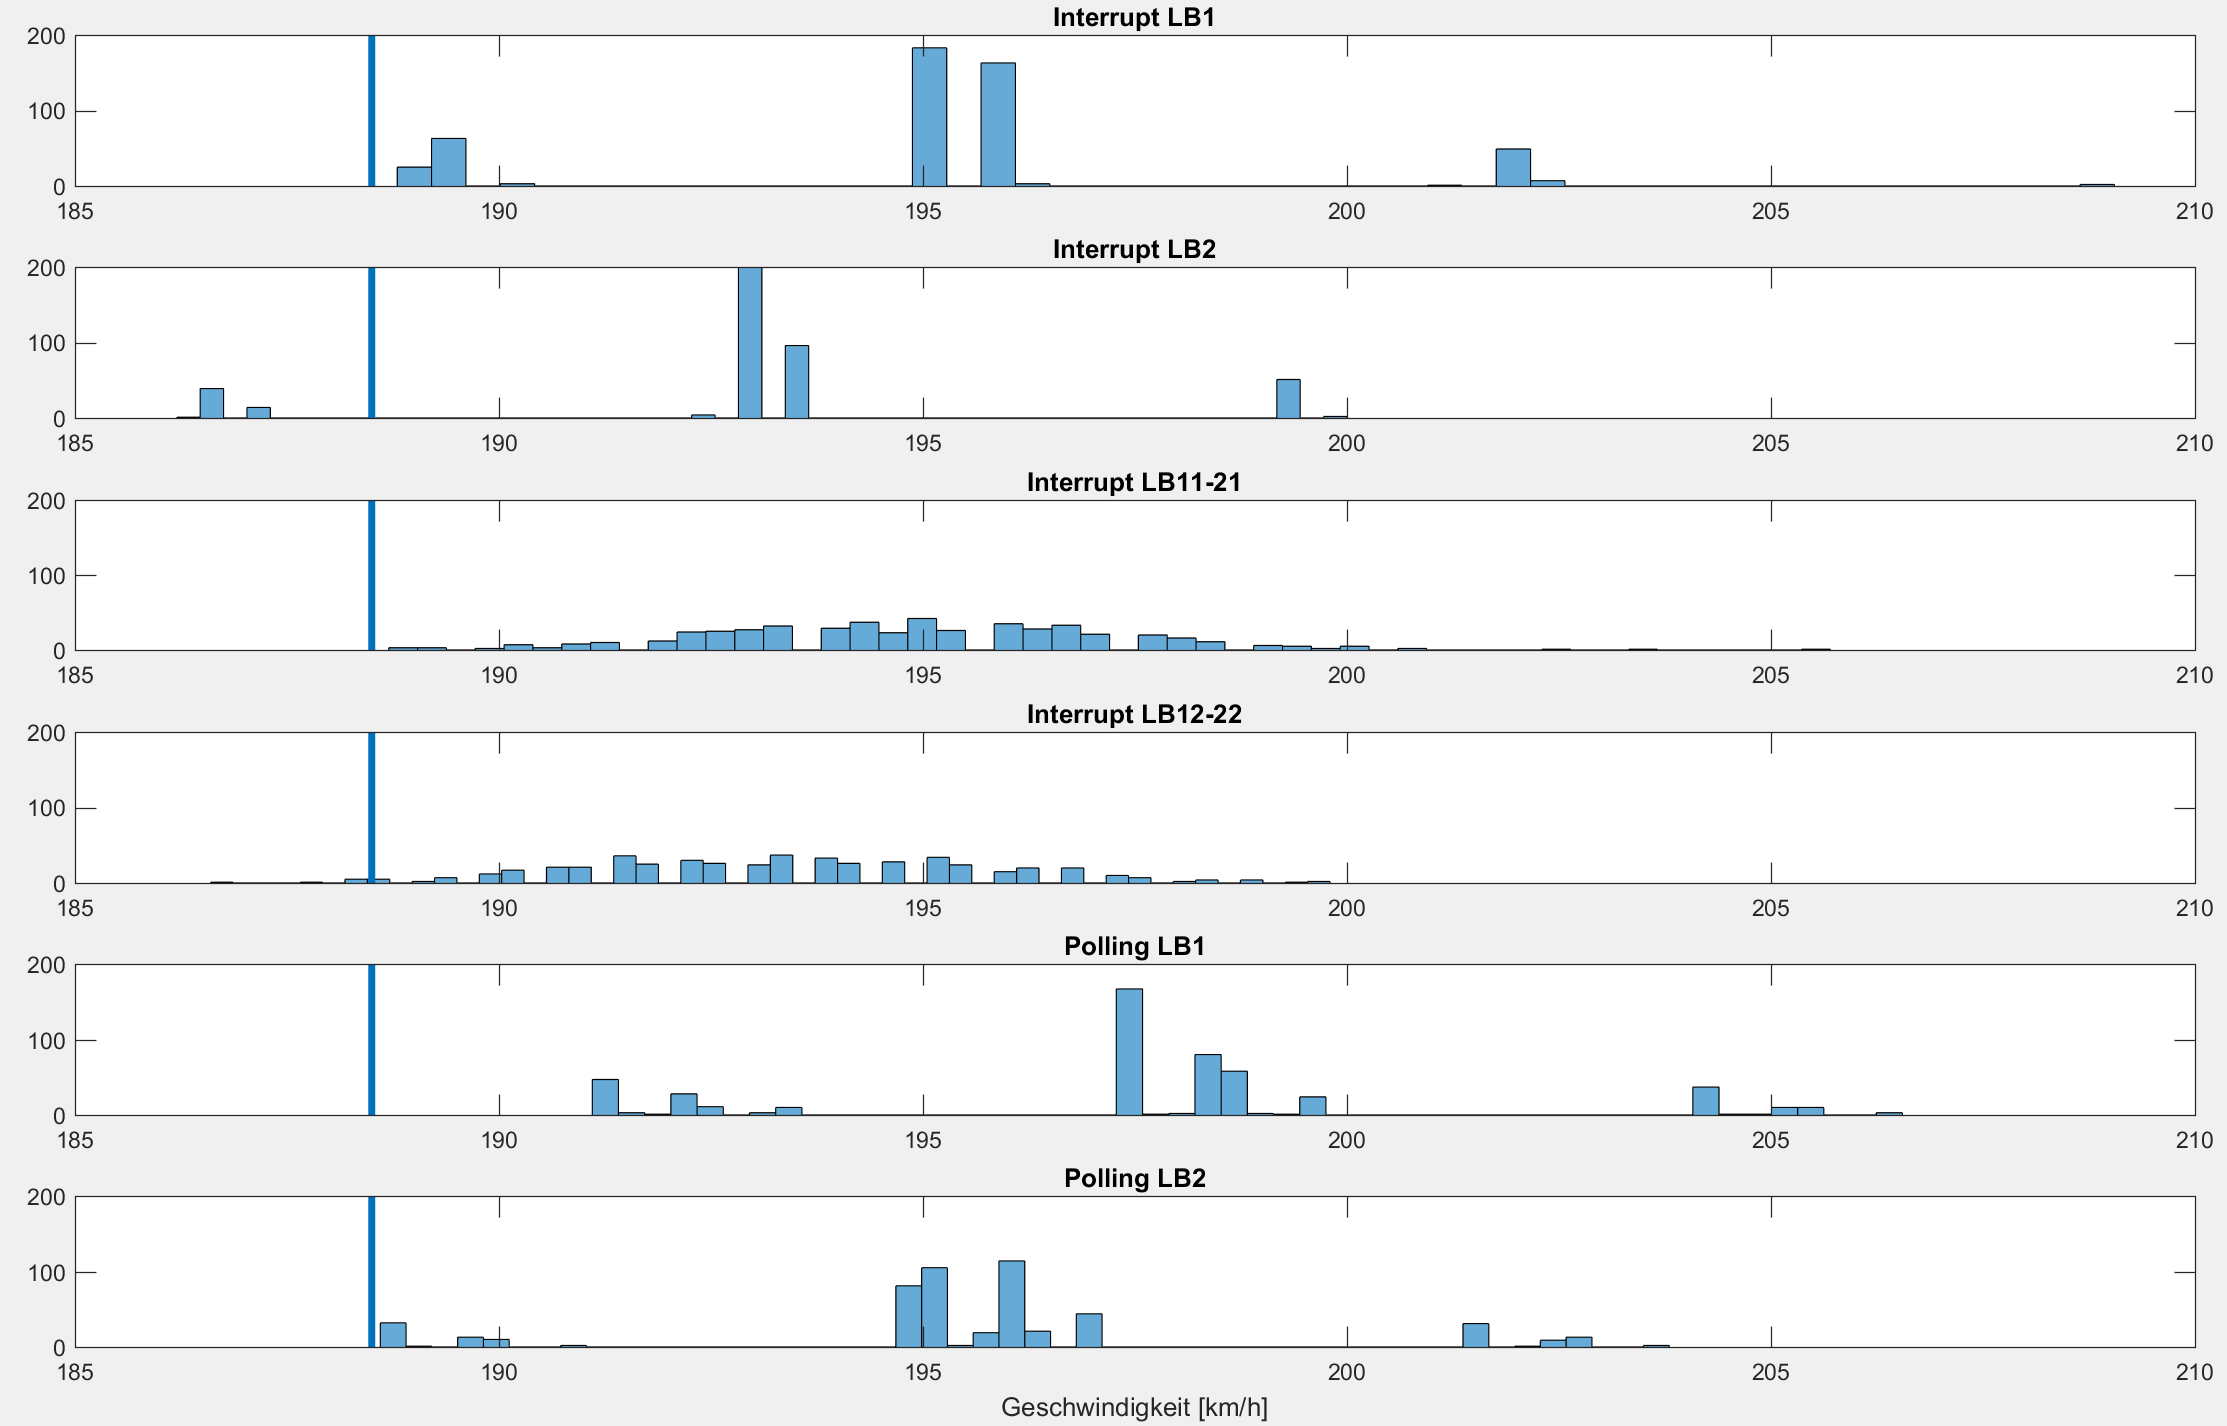
\includegraphics[width=\textwidth]{images/hist2000.png}
    \caption{Histogramm}
    \label{fig:Hist}
\end{figure}

\clearpage
%\begin{figure}[ht]
%    \centering
%    %    \missingfigure{Bild einfügen}
%    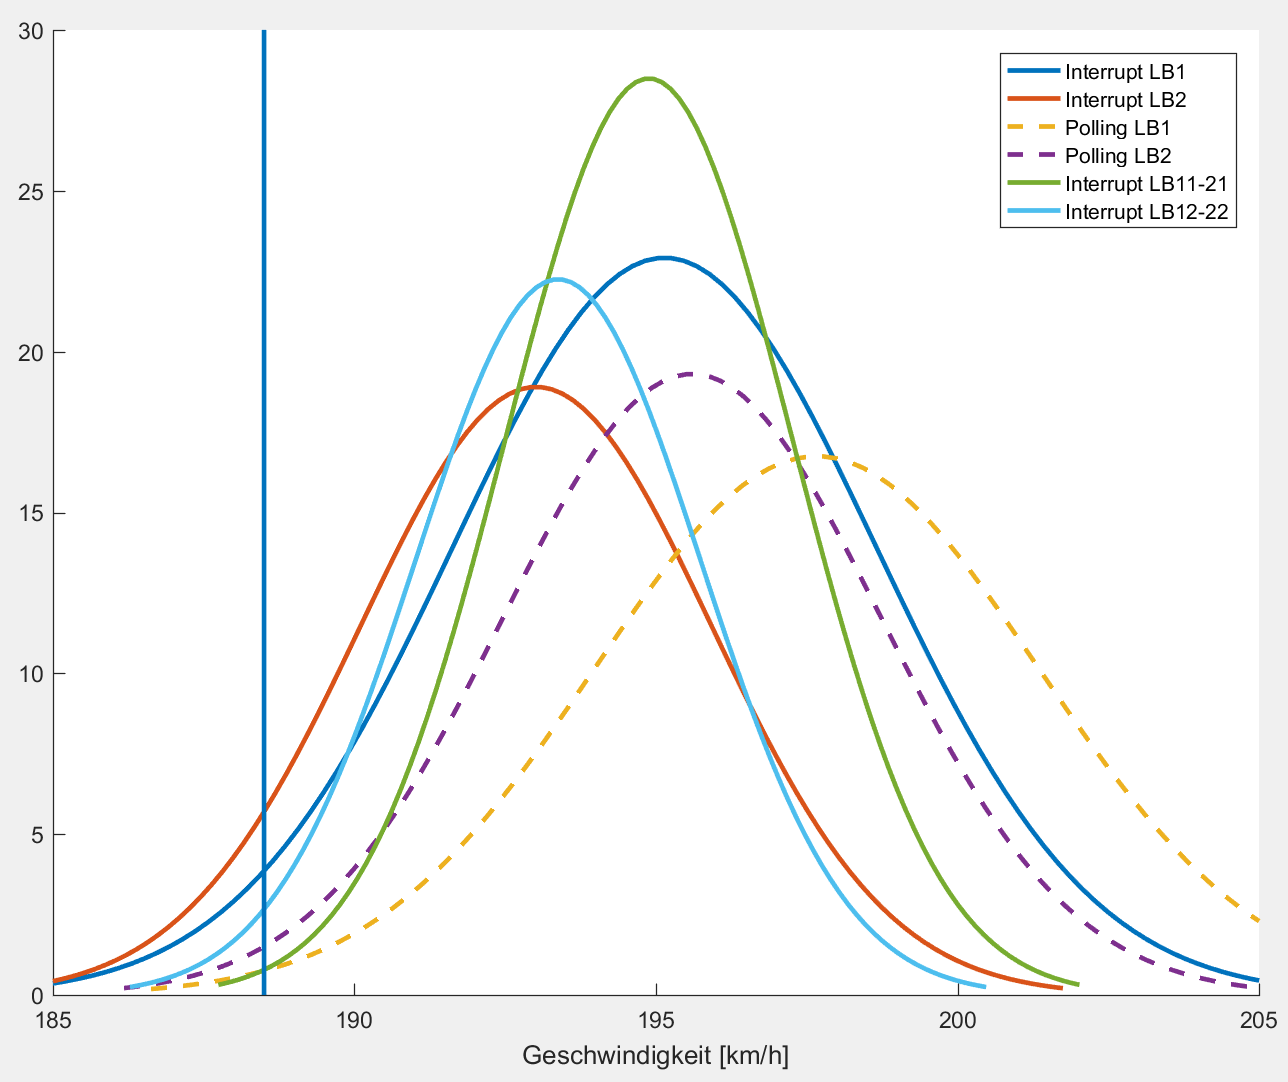
\includegraphics[width=\textwidth]{images/densi.png}
%    \caption{Dichteverteilung}
%    \label{fig:density}
%\end{figure}


%   IntLB1     IntLB2  IntLB1121  IntLB1222   PulsLB1   PulsLB2
%    1.8026    1.5088    1.2213    1.2238    1.8617    1.6057
\clearpage
\subsection{Fehlerquellen}
Die \ref{fig:AuswertungZeitfehler} zeigt den maximalen Geschwindigkeitsfehler wenn mit der maximalen Ansprechzeit der Lichtschranke von 0.5 ms gerechnet wird. Diese Abbildung soll vor allem verdeutlichen, dass Zeitfehler bei hohen Geschwindigkeiten stärker Gewichtet werden.

\begin{figure}[ht]
    \centering
    %    \missingfigure{Bild einfügen}
    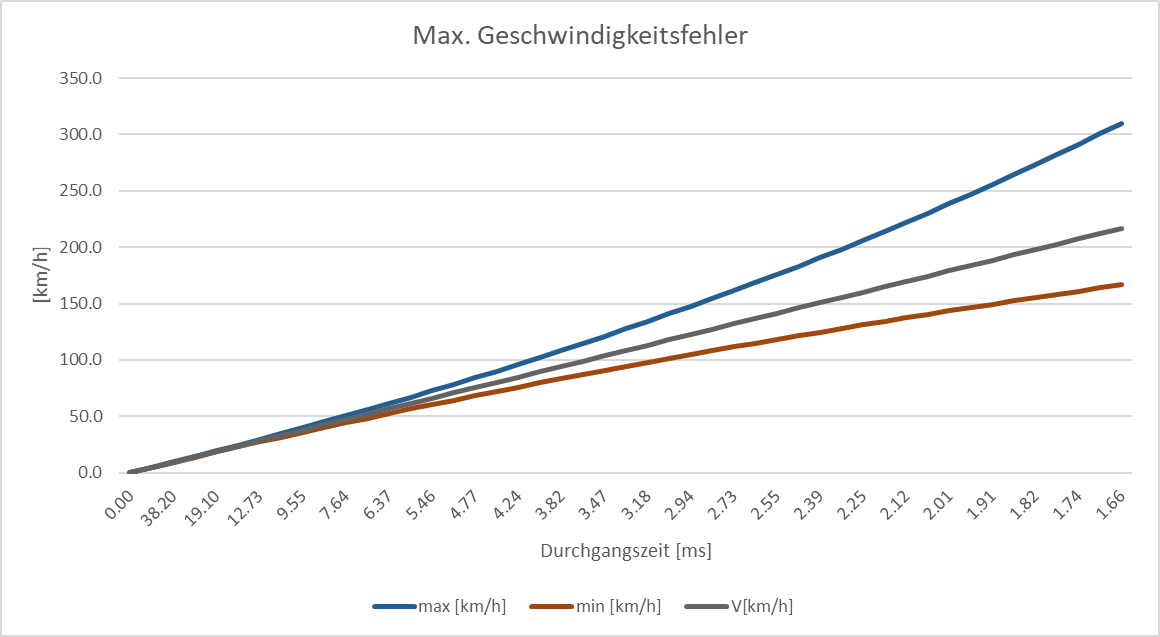
\includegraphics[width=\textwidth]{images/Zeitfehler.png}
    \caption{Max. Geschwindigkeitsfehler maximaler Ansprechverzögerung.}
    \label{fig:AuswertungZeitfehler}
\end{figure}

Die für diesen Versuchsaufbau relevanten \marg{Fehlerquellen}Fehlerquellen sind im Polling-Modus:
\begin{itemize}
    \item Ungenauer Abstand der Lichtschranken zum Drehpunkt des Rotors.
    \item Ungenauigkeit infolge unterschiedlicher Reaktionszeiten der Lichtschranke.
    \begin{itemize}
        \item Wiederholpräzision
        \item Hysterese
    \end{itemize}
    \item Ungenauigkeit infolge Regelabweichung des Motors.
    \item Ungenauigkeit infolge der Reaktionszeit des Arduinos.
\end{itemize}

Beim Interrupt-Modus kommt wegen dem Vergleich zwischen den Lichtschranken noch weitere Ungenauigkeiten dazu:
\begin{itemize}
    \item Ungenauer Abstand der Lichtschranken zueinander.
\end{itemize}
%\null \vspace{0.5\baselineskip}
Die Ungenauigkeit infolge unterschiedlicher Reaktionszeiten der beiden Lichtschranken kann evt. mit dem Aufsetzen einer Schlitzmaske, welche es als Zubehör gibt, auf kosten der Reichweite, noch verbessert werden. Dies würde sich positiv auf die Präzision auswirken. Für eine Verbesserung der Genauigkeit ist vor allem ein geometrisch genauerer Aufbau nötig. \\

Ein weiteres Problem ist, dass auf Grund des rotierenden Aufbaus nicht abschliessend gesagt werden kann, ob alle Durchläufe korrekt detektiert werden. Einzelne Durchläufe könnten nicht detektiert worden sein. Mit diesem Versuchsaufbau ist es jedoch nicht möglich einen einzelnen schnellen Durchgang zu erzeugen.


    \clearpage\pagebreak
    \section{Empfehlung}
Einige Fehler könnten mit einem genaueren Messaufbau eliminiert werden.
Die Genauigkeit von 5\% ist in den Augen des Verfassers ausreichend. Eine Verbesserung kann erzielt werden wenn die momentane Ausführung mit 2 Sensoren beibehalten wird und die erfassten Messwerte noch weiterverarbeitet werden. Vorstellbar wäre dabei die Bildung eines Medians um Ausreisser zu minimieren.\\

Jedoch zeigte der Vergleich der Implementationsmethoden, dass auch nur eine Lichtschranke ausreichend sein kann. Es empfiehlt sich dies weiter zu untersuchen.
    \clearpage\pagebreak
%	\section{Einleitung}


Lorem\marg{Ausgangssituation} Lorem dolor sit amet, consetetur sadipscing elitr, sed diam nonumy eirmod tempor invidunt ut labore et dolore magna aliquyam erat, sed diam voluptua. At vero eos et accusam et justo duo dolores et \autocite[22]{Roppel2006} ea rebum. Stet clita kasd gubergren, no sea \textbf{\ref{tab:Hochwasserszenarien}} takimata sanctus est Lorem ipsum dolor sit amet. Lorem ipsum dolor sit amet, consetetur sadipscing elitr, sed diam nonumy eirmod tempor invidunt ut labore et dolore magna aliquyam erat, sed diam voluptua. At vero eos et accusam et justo duo dolores et ea rebum. Stet clita kasd gubergren, \textbf{\ref{fig:HSR}} no sea takimata sanctus est Lorem ipsum dolor sit\footcite{Roppel2006} \textbf{\ref{eq:Hochwasserzufluss}} amet.\footfullcite{Roppel2006}

\begin{figure}[ht]
	\centering
	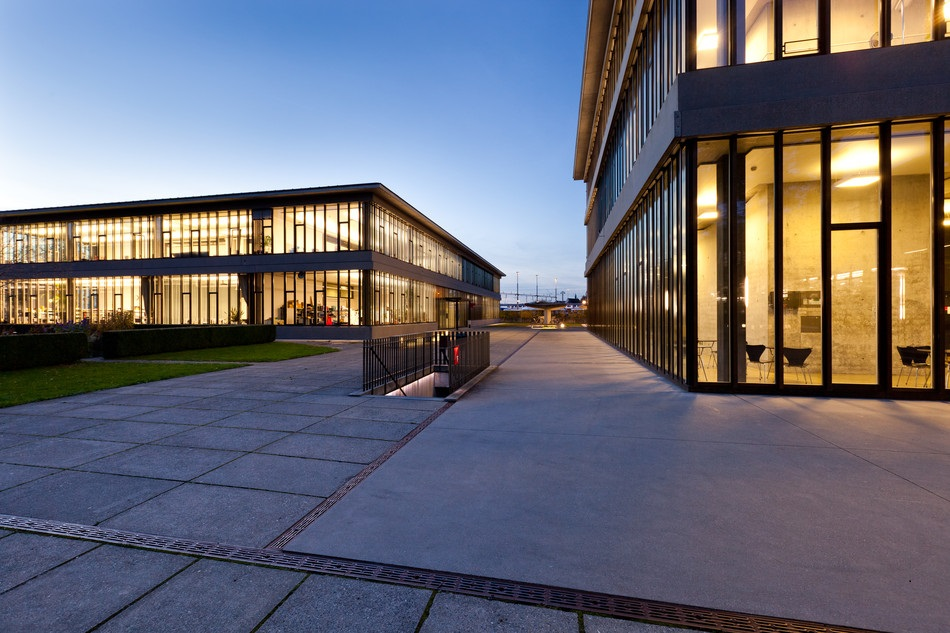
\includegraphics[width=0.6\textwidth]{images/hsr.jpg}
	\caption{\acs{HSR} \autocite{IR}}
	\label{fig:HSR}
\end{figure}

Lorem\marg{Was ist das Problem?}

 \begin{equation}\label{eq:Hochwasserzufluss}
\frac{Q(t)}{Q_{max}} = \left(\frac{t}{t_max}\cdot e^{1-\frac{t}{t_max}} \right)^n
\end{equation}
\myequations{Definition Hochwasserzufluss}

\begin{table}[ht]
    \centering
	\begin{tabular}{|l|l|l|l|l|l|}
		\hline 
		\textbf{Ganglinie}	&\textbf{[ ... ]}  	& \textbf{A} 	 & \textbf{B}  	& \textbf{C} 	& \textbf{D}  \\ 
		\hline 
		$ Q_{max} $			& $ m^3/s $ 		& 50 			& 70		  	& 180			& 540 \\ 
		\hline 
		$ t_{max} $			& $ h $ 			& 2  			& 2 			& 3 			& 4 \\ 
		\hline 
		n					& --  				& 6  			& 6 			& 6 			& 6  \\ 
		\hline 
	\end{tabular} 
	\caption{Hochwasserszenarien}\label{tab:Hochwasserszenarien}
\end{table}

Lorem \marg{Ziel} Lorem dolor sit amet, consetetur sadipscing elitr, sed diam nonumy ei\\

Lorem \marg{Wie soll das Problem gelöst werden?} Lorem dolor sit amet, consetetur sadipscing elitr, sed diam nonumy ei \\
\ac{HSR}\\
\acs{HSR}\\
\acl{HSR}


\clearpage
%	\pagebreak
%    \section{Einleitung}


Lorem\marg{Ausgangssituation} Lorem dolor sit amet, consetetur sadipscing elitr, sed diam nonumy eirmod tempor invidunt ut labore et dolore magna aliquyam erat, sed diam voluptua. At vero eos et accusam et justo duo dolores et \autocite[22]{Roppel2006} ea rebum. Stet clita kasd gubergren, no sea \textbf{\ref{tab:Hochwasserszenarien}} takimata sanctus est Lorem ipsum dolor sit amet. Lorem ipsum dolor sit amet, consetetur sadipscing elitr, sed diam nonumy eirmod tempor invidunt ut labore et dolore magna aliquyam erat, sed diam voluptua. At vero eos et accusam et justo duo dolores et ea rebum. Stet clita kasd gubergren, \textbf{\ref{fig:HSR}} no sea takimata sanctus est Lorem ipsum dolor sit\footcite{Roppel2006} \textbf{\ref{eq:Hochwasserzufluss}} amet.\footfullcite{Roppel2006}

\begin{figure}[ht]
	\centering
	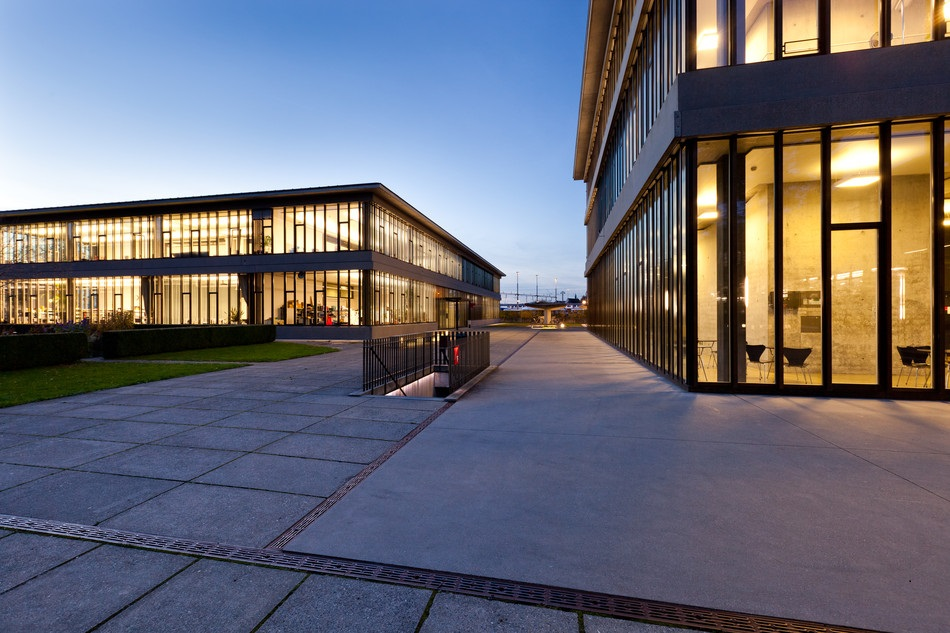
\includegraphics[width=0.6\textwidth]{images/hsr.jpg}
	\caption{\acs{HSR} \autocite{IR}}
	\label{fig:HSR}
\end{figure}

Lorem\marg{Was ist das Problem?}

 \begin{equation}\label{eq:Hochwasserzufluss}
\frac{Q(t)}{Q_{max}} = \left(\frac{t}{t_max}\cdot e^{1-\frac{t}{t_max}} \right)^n
\end{equation}
\myequations{Definition Hochwasserzufluss}

\begin{table}[ht]
    \centering
	\begin{tabular}{|l|l|l|l|l|l|}
		\hline 
		\textbf{Ganglinie}	&\textbf{[ ... ]}  	& \textbf{A} 	 & \textbf{B}  	& \textbf{C} 	& \textbf{D}  \\ 
		\hline 
		$ Q_{max} $			& $ m^3/s $ 		& 50 			& 70		  	& 180			& 540 \\ 
		\hline 
		$ t_{max} $			& $ h $ 			& 2  			& 2 			& 3 			& 4 \\ 
		\hline 
		n					& --  				& 6  			& 6 			& 6 			& 6  \\ 
		\hline 
	\end{tabular} 
	\caption{Hochwasserszenarien}\label{tab:Hochwasserszenarien}
\end{table}

Lorem \marg{Ziel} Lorem dolor sit amet, consetetur sadipscing elitr, sed diam nonumy ei\\

Lorem \marg{Wie soll das Problem gelöst werden?} Lorem dolor sit amet, consetetur sadipscing elitr, sed diam nonumy ei \\
\ac{HSR}\\
\acs{HSR}\\
\acl{HSR}


\clearpage
%    \pagebreak
%	\section{Pflichtenheft}
Lorem\marg{Ausgangslage} \todo{Abstract} ipsum dolor sit amet, consetetur sadipscing elitr, sed diam nonumy eirmod tempor invidunt ut labore et dolore magna aliquyam erat, sed diam voluptua. At vero eos et accusam et justo duo dolores et ea rebum. Stet clita kasd gubergren, no sea takimata sanctus est Lorem ipsum dolor sit amet. Lorem ipsum dolor sit amet, consetetur sadipscing elitr, sed diam nonumy eirmod tempor invidunt ut labore et dolore magna aliquyam erat, sed diam voluptua. At vero eos et accusam et justo duo dolores et ea rebum. Stet clita kasd gubergren, no sea takimata sanctus est Lorem ipsum dolor sit amet.
\subsection{Bestandesaufnahme}
dd\marg{Ausgangslage}ff
\missingfigure{Test}
\subsubsection{Funktionsweise des Systems}
dd\marg{Ausgangslage}ff
\subsection{Anforderungen an das System}
dd\marg{Ausgangslage}ff
\subsubsection{Funktionsablauf}
dd\marg{Ausgangslage}ffv
v
\clearpage
%    \pagebreak
%    \section{Pflichtenheft}
Lorem\marg{Ausgangslage} \todo{Abstract} ipsum dolor sit amet, consetetur sadipscing elitr, sed diam nonumy eirmod tempor invidunt ut labore et dolore magna aliquyam erat, sed diam voluptua. At vero eos et accusam et justo duo dolores et ea rebum. Stet clita kasd gubergren, no sea takimata sanctus est Lorem ipsum dolor sit amet. Lorem ipsum dolor sit amet, consetetur sadipscing elitr, sed diam nonumy eirmod tempor invidunt ut labore et dolore magna aliquyam erat, sed diam voluptua. At vero eos et accusam et justo duo dolores et ea rebum. Stet clita kasd gubergren, no sea takimata sanctus est Lorem ipsum dolor sit amet.
\subsection{Bestandesaufnahme}
dd\marg{Ausgangslage}ff
\missingfigure{Test}
\subsubsection{Funktionsweise des Systems}
dd\marg{Ausgangslage}ff
\subsection{Anforderungen an das System}
dd\marg{Ausgangslage}ff
\subsubsection{Funktionsablauf}
dd\marg{Ausgangslage}ffv
v
\clearpage
%	\pagebreak
%	 \vspace{-3cm}
\section{Projektplan}
%{\centering
%	\vspace{-0.4cm}}
%	\includegraphics[angle=90,clip, trim= 0.5cm 5.5cm 1cm 2cm, scale=0.83]{sections/Projektterminplan_SA.pdf}\par}

%	\pagebreak
%	\section{Hauptstudie}
%	\pagebreak
%	\section{Fazit}
%	\pagebreak

\newgeometry{left=2cm,right=2cm,top=1cm,bottom=1cm,headsep=1.5cm, marginparwidth=1mm,marginparsep=3mm,includeheadfoot}	
%	\section{Erklärung zur Urheberschaft}
\vspace{0.8cm}
\textbf{Erklärung}\\

Wir erklären hiermit an Eides statt, dass ich die vorliegende Arbeit ohne Benutzung anderer als der angegebenen Hilfsmittel erstellt habe; die aus fremden Quellen direkt oder indirekt übernommenen Gedanken sind als solche kenntlich gemacht. Die Arbeit wurde bisher in gleicher oder ähnlicher Form keiner anderen Prüfungsbehörde vorgelegt und auch noch nicht veröffentlicht.\\
\vspace{0.8cm}\\

\begin{tabular}{l l}
    \textbf{Ort} & \textbf{Datum} \\
    \Place  & \today
\end{tabular}
\vspace{0.8cm}

\textbf{Unterschrift}\\
\vspace{0.2cm}
\AuthorOne \hspace{3cm} \AuthorTwo

\clearpage


%	\pagebreak
%	\section{Verzeichnisse}
%Abkürzungsverzeichniss, für schön ausrichten längste Abkürzung in eckige Klammer
\subsection{Abkürzungen}
\vspace{0.1cm}
\begin{acronym}[BA]
%\acro{Abkürzung}{Ausdruck ausgeschrieben}	
\acro{HSR}{Hochschule für Technik Rapperswil}
\end{acronym}	
\clearpage
\pagebreak


%Gleichungsverzeichnis
\subsection{\listequationsname}
\renewcommand*\listequationsname{}
\listofmyequations\thispagestyle{fancy}
\clearpage
\pagebreak

%Abbildungsverzeichnis
\subsection{\listfigurename}
\renewcommand*\listfigurename{}
\listoffigures\thispagestyle{fancy}
\clearpage
\pagebreak

%Tabellenverzeichnis
\subsection{\listtablename}
\renewcommand*\listtablename{}
\listoftables\thispagestyle{fancy}
\clearpage
\pagebreak

%Quellenverzeichnis
\subsection{Quellenverzeichnis}
\printbibliography[heading=subbibliography,keyword=lit, title={Literaturquellen}]
\printbibliography[heading=subbibliography,keyword=manual, title={Datenblätter}]
\printbibliography[heading=subbibliography,keyword=online, title={Onlinequellen}]
\printbibliography[heading=subbibliography,keyword=abb, title={Bildquellen}]

\clearpage
%	\clearpage
%	\pagebreak
	\pagestyle{appendix}
	\section*{Anhang}
\addcontentsline{toc}{section}{Anhang}
\appendix
\startcontents[sections]
\printcontents[sections]{l}{1}{\setcounter{tocdepth}{2}}
\clearpage
\pagebreak


%\includepdf[pages={1},scale=0.95, pagecommand={\section{Anhangbsp mit PDF}},offset=0 -2cm]{sections/anhang/BA.pdf}
%\includepdf[pages={2-},scale=0.95, pagecommand={\thispagestyle{appendix}}]{sections/anhang/BA.pdf}

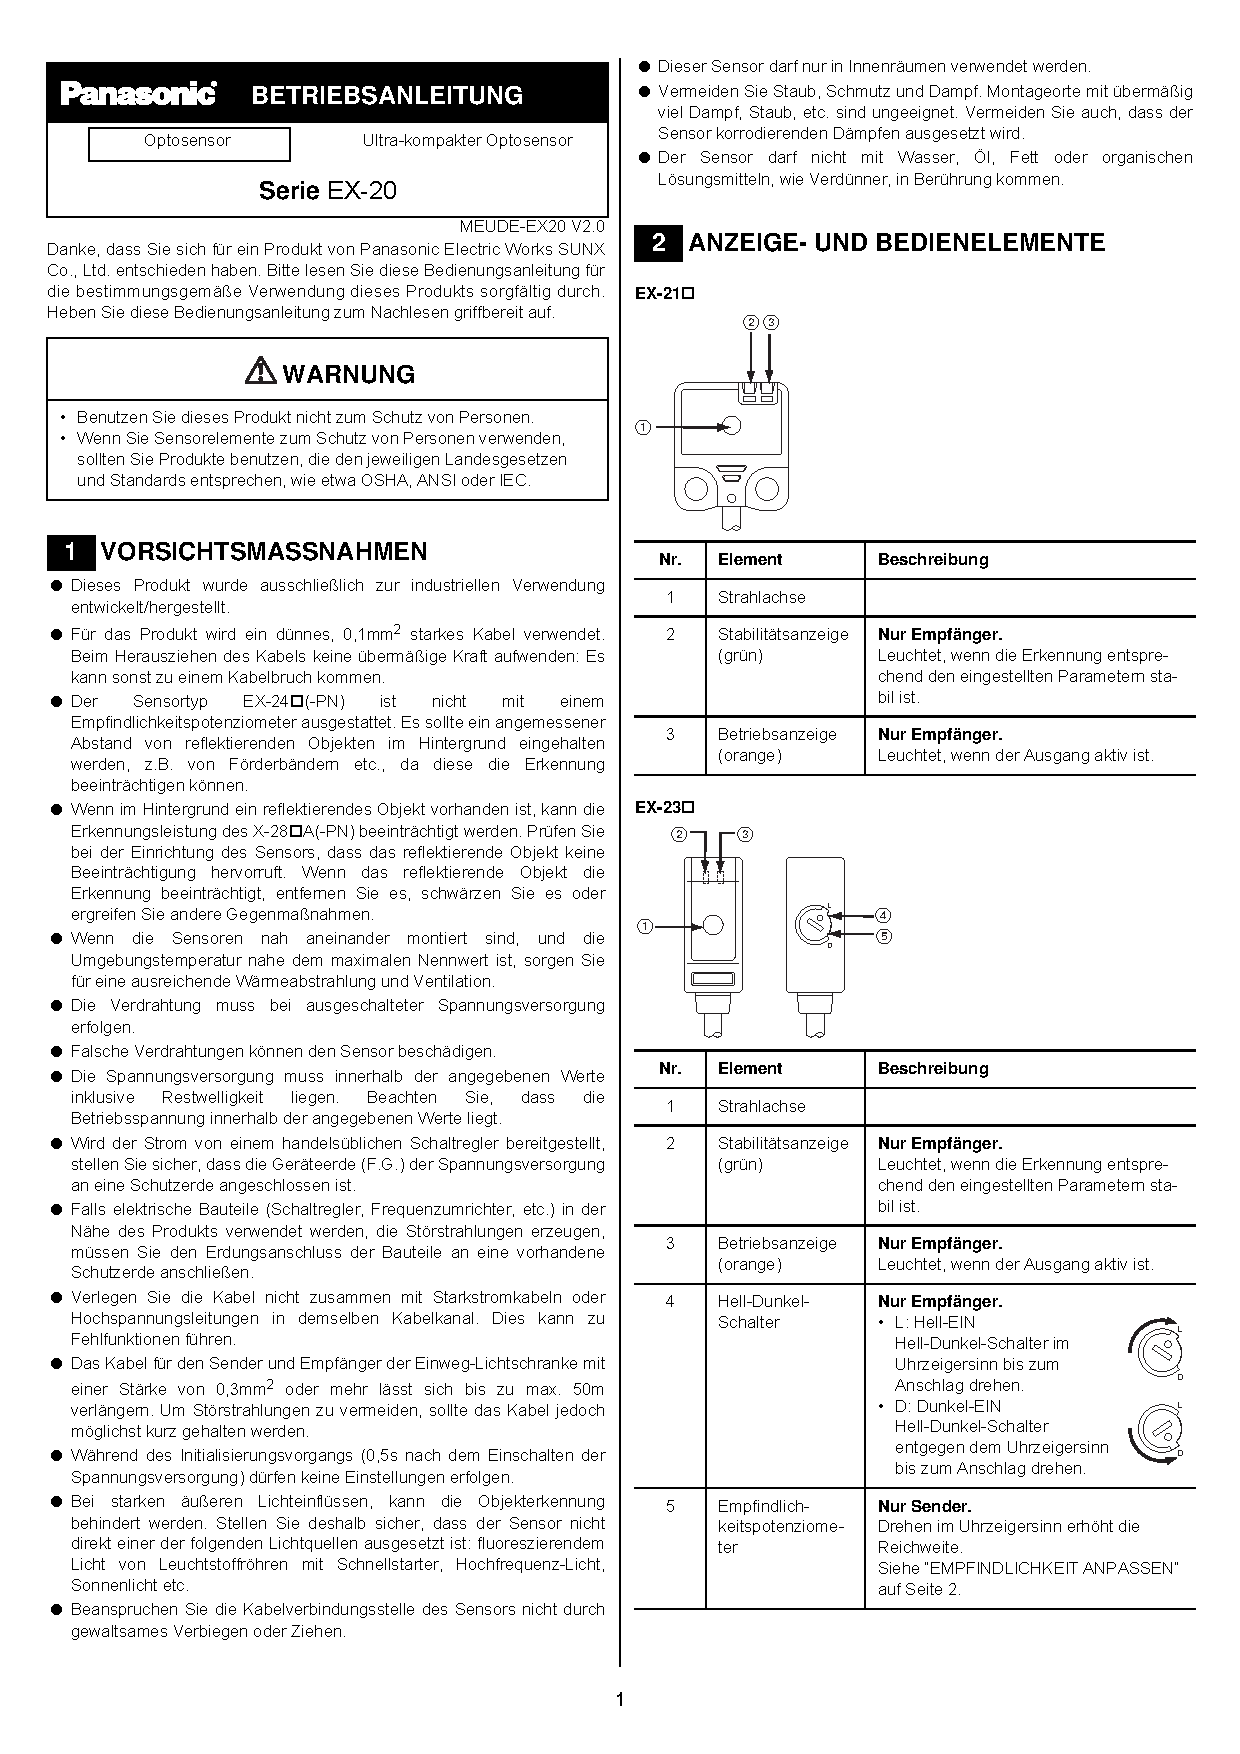
\includepdf[pages={1},scale=0.85, pagecommand={\section{Datenblatt Panasonic EX-20}\label{app:ex20}},offset=0 -2cm]{sections/anhang/ex20_ger_man.pdf}
\includepdf[pages={2-},scale=0.92, pagecommand={\thispagestyle{appendix}}]{sections/anhang/ex20_ger_man.pdf}


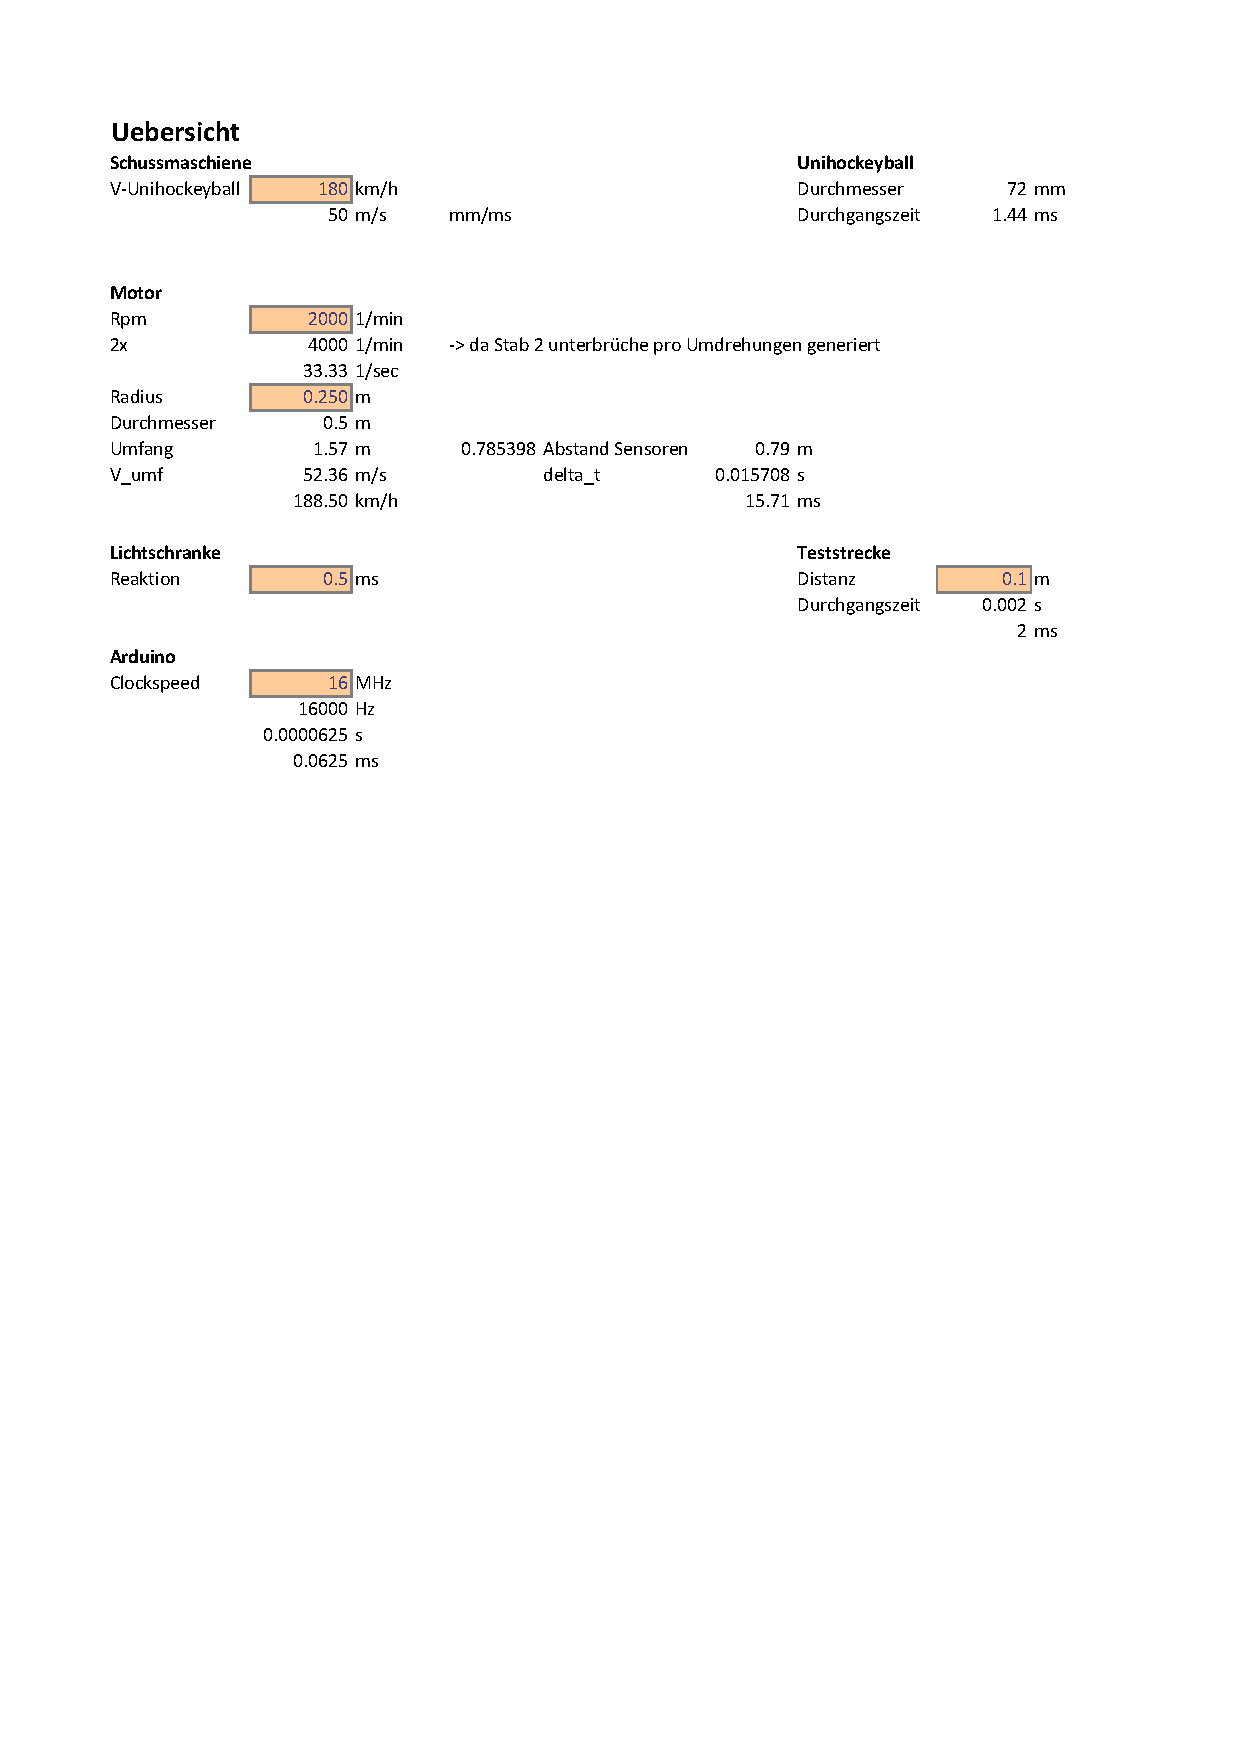
\includepdf[pages={1},scale=0.95, pagecommand={\section{Berechnungen}\label{app:berechnung}},offset=0 -2cm]{sections/anhang/Berechnungen.pdf}
\includepdf[pages={2-},scale=0.95, pagecommand={\thispagestyle{appendix}}]{sections/anhang/Berechnungen.pdf}

\section{Arduinoprogramm}\label{app:ardprog}
\lstinputlisting[style=customc++]{src/BWMvelocity.cpp}

\section{Python}\label{app:python}
\lstinputlisting[style=python]{src/ReadSerial.py}

\section{Auswertung}\label{app:Auswertung}
\includegraphics[width=\textwidth]{images/auswertungLS1.png}\\
\includegraphics[width=\textwidth]{images/auswertungLS2.png}\\
\includegraphics[width=\textwidth]{images/auswertungLS1LS2.png}\\
\includegraphics[width=\textwidth]{images/auswertungInt.png}\\

\includegraphics[width=\textwidth]{images/auswertungSpeed.png}\\
	\cleardoublepage
\end{document}
